% (c) 2012 -2014 Dimitrios Vrettos - d.vrettos@gmail.com
% (c) 2014 Claudio Carboncini - claudio.carboncini@gmail.com
% (c) 2014 Daniele Zambelli - daniele.zambelli@gmail.com

\input{\folder naturali_grafici.tex}

\chapter{Numeri naturali}

\inicapitolo{
\begin{itemize}
\item i numeri naturali;
\item l'importante strumento matematico costituito dalle funzioni;
\item i grafi ad albero;
\item le operazioni con i naturali e le loro proprietà;
\item le proprietà delle potenze;
\item le espressioni con i numeri naturali;
\item i numeri primi;
\item la divisibilità, i divisori e i multipli.
\end{itemize}
}

\section{L'origine dei numeri}
\label{sec:nat_origine}

L'origine del sistema dei numeri naturali si perde nella notte dei tempi. 
Non abbiamo documenti sufficienti per capire come l'uomo li abbia 
costruiti o scoperti; è possibile che il nostro sistema di numerazione 
sia nato contemporaneamente al linguaggio stesso della specie umana. 
Sono stati ritrovati reperti fossili risalenti a più di trentamila
anni fa, recanti delle incisioni a distanza regolare. 
In particolare, è stato ritrovato un osso di babbuino, 
detto ``Osso di Ishango''
\footnote{\url{http://it.wikipedia.org/wiki/Osso_d'Ishango}} 
in quanto è stato rinvenuto presso la città di Ishango nel Congo tra il 
Nilo e il lago Edoardo, che riporta delle tacche disposte in modo tale da 
farci pensare che rappresentino dei numeri o dei calcoli. 
L'osso risale a circa~20\,000 anni fa.

\vspace{.25em}
\affiancati{.56}{.42}{
Possiamo immaginare che i pastori per contare i capi del proprio gregge, 
facessero delle tacche su dei bastoni mano a mano che le pecore entravano 
nel recinto una alla volta: una tacca per ogni pecora. 
Tuttavia, questo metodo di associazione uno a uno (una tacca per una 
pecora) non è efficace per greggi, o gruppi di oggetti, di grandi 
dimensioni. 
Si immagini, per esempio, la difficoltà di tracciare cinquecento tacche su 
un bastone. 
}{
\immagine[.30]{Testo alternativo figura: osso con incise alcune tacche 
regolari.}
{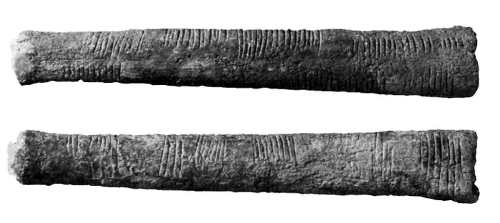
\includegraphics{img/fig001.png}}
}

\vspace{.25em}
È possibile allora che, per rappresentare numeri grandi, si siano 
cominciati a usare simboli specifici che richiamassero alla mente i 
numeri grandi e che contemporaneamente siano state fissate alcune 
regole per associare questi simboli.

Sappiamo per certo che circa~6\,000 anni fa gli antichi Egizi scrivevano, 
incidendo sulla pietra, i numeri utilizzando geroglifici per le potenze 
di~10:

\vspace{-2ex}
\immagine[.6]
{Testo alternativo figura: geroglifici che rappresentano le potenze di 10 
da uno a un milione. 
In particolare
1 è rappresentato da una barretta verticale; 
10 come una U rovesciata; 
100 come un segmento in diagonale con in cima verso destra un ricciolo; 
1000 come una freccia verso il basso con alla base un piccolo triangolo e 
in cima una mezzaluna; 
10000 come un bastoncino verticale internamente bianco e sulla parte 
superiore leggermente inclinata verso destra di colore nero; 
100000 come una specie di pappagallo e 
infine 1000000 come un egiziano inginocchiato con una gamba ed entrambe 
le braccia aperte ed alzate verso il cielo.}
{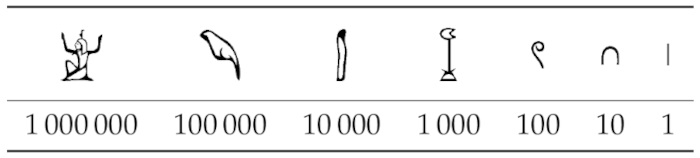
\includegraphics{img/hieropotdieci.png}}

\vspace{-2ex}
Ripetendo questi simboli è possibile scrivere, per esempio, il numero~3673 
così:

\vspace{-2ex}
\immagine[.35]
{Testo alternativo figura: numero 3673 scritto con i geroglifici e quindi 
usando i simboli descritti sopra e quindi n. 3 simboli della
``mezzaluna'', n. 6 simboli del ``ricciolo'', n. 7 simboli con la 
U rovesciata ed infine n. 3 barrette verticali.}
{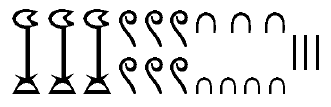
\includegraphics{img/hiero3673.png}}
\vspace{-2ex}

I Romani per rappresentare i numeri usavano sette lettere maiuscole: 
\(I=1\), \(V=5\), \(X=10\), \(L=50\), \(C=100\), \(D=500\), 
\(M=1000\).
Il numero~\(MM\) rappresenta~\(~1000+1000 =~2000\); il numero~\( VI\) 
rappresenta~\(~5+1=6~\), mentre il numero~\( IV~\) rappresenta~\(~5-1=4~\).

Nel medioevo si diffuse anche in Italia, e poi in Europa, la notazione 
usata dagli arabi di allora che a loro volta l'avevano appresa dagli 
abitanti dell'India. 
Non fu un passaggio facile: le cifre arabe richiesero alcuni secoli per 
essere accettate dagli europei e soppiantare i simboli romani.

\section{I numeri naturali}
\label{sec:nat_naturali}

I primi numeri che abbiamo usato sin da bambini per contare gli oggetti o 
le persone si chiamano \emph{numeri naturali}
\[0,\quad 1,\quad 2,\quad 3,\quad 4,\quad 5,\quad 6,\quad 7,\quad 8,\quad 
  9,\quad 10,\quad 11,\quad 12,\quad 13,\quad \dots\]
L'insieme di tutti questi numeri si indica con la lettera~\(\N\).

Cosa hanno in comune le dita di una mano, con~5 mele,~5~penne,~5~sedie? 
Evidentemente il numero~5. Una caratteristica cioè che è comune a tutti i 
gruppi formati da~5 oggetti. 
Questa caratteristica può essere vista come un oggetto a sé stante, 
un oggetto astratto di tipo matematico.

Ma i numeri naturali non servono solo per indicare quanti oggetti ci sono 
(aspetto \emph{cardinale} \ind{cardinali} del numero), vengono usati 
anche per rappresentare 
l'ordine con cui si presentano gli oggetti, (aspetto \emph{ordinale} 
\ind{ordinali}), 
l'ordine per esempio con cui i corridori arrivano al traguardo: primo, 
secondo, terzo, \ldots

Nonostante i numeri naturali e le operazioni su di essi ci vengano 
insegnati fin da piccoli e nonostante l'umanità li usi da tempi 
antichissimi, una loro piena comprensione non è semplice, come dimostra 
il fatto che ancora oggi ci siano dei problemi aperti relativi a questi 
numeri. 
Il dibattito su cosa sono i numeri e su cosa si fondano è stato 
particolarmente animato nei primi decenni del \(XX\)~secolo, quando ne 
hanno discusso matematici e filosofi come Frege, Peano, Russell, Hilbert e 
tanti altri. 
Oggi ci sono diversi punti di vista.


\section{Cosa sono}
\label{sec:nat_definizione}

I numeri naturali sono alla base dell'aritmetica, 
tutti gli altri numeri si possono costruire a partire da questi. 
Tutti noi abbiamo una idea di cosa siano i numeri naturali e, in generale, 
in questo testo ci riferiremo a questa idea ingenua di numeri naturali.

Ci sono diversi modi per definirli a partire da concetti più primitivi 
come, ad esempio, gli \emph{insiemi} o da \emph{assiomi}.
Di seguito sono presentati gli assiomi di Peano\footnote{
Vedi \url{https://it.wikipedia.org/wiki/Assiomi_di_Peano}}
che permettono di definire i numeri naturali a partire da due concetti 
primitivi e da 5 assiomi\ind{assiomi di Peano}, cioè affermazioni su cui 
siamo d'accordo.

I concetti primitivi per definire i numeri naturali sono:

\begin{itemize}[noitemsep]
\item lo zero;
\item il successore di un numero.
\end{itemize}

Lo \emph{zero}\ind{zero} è il numero che serve per contare gli elementi 
di un gruppo con il minore numero di oggetti possibile: un gruppo vuoto.

Il \emph{successore}\ind{successore} di un numero naturale~\(n\) è quel 
numero che viene subito dopo~\(n\) e che rappresenta il numero di 
oggetti di un gruppo quando se ne aggiunge uno.

Le seguenti affermazioni possono quindi individuare i numeri naturali:

\begin{enumerate}[noitemsep]
\item Zero è un numero naturale.
\item Per ogni numero naturale, anche il suo successore è un numero 
naturale.
\item Numeri diversi hanno successori diversi.
\item Lo zero non è successore di nessun numero naturale.
\item Se una proprietà vale per lo zero e, 
valendo per un numero naturale qualsiasi, 
vale anche per il suo successore, 
allora vale per ogni numero naturale.
\end{enumerate}

In pratica i numeri naturali sono la sequenza:

zero,\quad uno,\quad due,\quad tre,\quad \dots,\quad
centoventitre,\quad centoventiquattro,\quad 
\dots

Un modo comodo per esprimere qualunque numero naturale è usare dei segni 
appositi, le cifre, e un sistema per rappresentarli:

0,\quad 1,\quad 2,\quad 3,\quad \dots,\quad 123,\quad 124, \dots

\section{Il sistema di numerazione decimale posizionale}
\label{sec:nat_sist10}

Il modo di scrivere i numeri dei romani risultava piuttosto complicato sia 
nella scrittura dei numeri sia nell'esecuzione dei calcoli. 
Il sistema moderno di scrittura dei numeri fa uso dei soli dieci 
simboli:\quad 0,\quad 1,\quad 2,\quad 3,\quad 4,\quad 5,\quad 
6,\quad 7,\quad 8,\quad 9,\quad che vengono detti \emph{cifre}\ind{cifra}.
Un numero può essere rappresentato da una sequenza ordinata di cifre, 
anche ripetute.

Per rappresentare il numero dieci che segue il~9 non si fa uso di un 
simbolo diverso ma si scrivono due cifre: il simbolo~1 a sinistra e il 
simbolo~0 a destra. 
Per chiarire questo metodo utilizziamo un pallottoliere con aste 
verticali capaci di contenere fino a~9 dischetti: 
un'asta vuota rappresenta la cifra zero, aggiungendo dischetti possiamo 
arrivare alla cifra 9 e così abbiamo riempito tutta un'asta. 
Se vogliamo aggiungere ancora un dischetto, svuotiamo tutta l'asta e ne 
mettiamo uno sull'asta più a sinistra.
Il numero successore del nove viene così rappresentato da un \emph{uno} 
seguito da uno \emph{zero}.

\affiancati{.39}{.59}{
I dischetti sull'ultima asta rappresentano il numero~9; un dischetto sulla 
penultima rappresenta il numero dieci:~10. 
Un dischetto sulla terzultima rappresentare il numero cento:~100.
In questo modo possiamo rappresentare tutti i numeri.
}{
\immagine[.65]
{Testo alternativo figura: 2 pallottolieri con 3 aste ciascuno, il primo 
con 9 dischetti nella terza asta e il secondo con un dischetto nella 
seconda asta (quella centrale).}
{\pallottoliere}
}

% \vspace{-.5em}
Le potenze di~10 sono importanti nel sistema decimale poiché 
rappresentano il peso di ciascuna cifra di cui è composto il numero. 
Nel pallottoliere ciascuna asta indica una potenza di dieci. 
Il valore di un numero si ottiene moltiplicando ciascuna cifra per il
suo peso e sommando i valori ottenuti.

Tre dischetti nella terza asta rappresentano tre centinaia, 
cioè il numero~\(~3 \cdot 10^2=300\).
Il numero~\(479\) significa quattro centinaia più sette decine più 
nove unità:~\(~4 \cdot 10^2 + 7 \cdot 10 + 9\).

Per quanto detto, il sistema di numerazione che usiamo è:

\begin{itemize} [noitemsep]
\item \emph{decimale} o a base dieci, 
perché usiamo dieci segni (cifre) per scrivere i numeri;
\item \emph{posizionale} 
perché una stessa cifra assume un peso (valore) diverso a seconda della 
posizione che occupa.
\end{itemize}

\subsection{Rappresentazione geometrica}
I numeri naturali possono essere rappresentati su una semiretta: 
si identifica il numero~0 con l'origine della semiretta, 
i numeri aumentano allontanandosi dall'origine e si deve scegliere un 
segmento che rappresenti un passo unitario.
Partendo dall'origine, a ogni passo si va al numero successivo.

% \vspace{-.5em}
\immagine[.8]
{Testo alternativo figura: semiretta orientata (orizzontale) con freccia 
verso destra con origine 0 e con unità pari ad 1.}
{\natrappgeo}

\vspace{-.5em}
Ogni numero naturale si costruisce a partire dal numero~0 e passando di 
volta in volta al numero successivo:~1 è il \indt{successore} di~0,~2~è il 
successore di~1,~3~è il successore di~2, etc. 
Ogni numero naturale ha il successore e ogni numero, a eccezione 
di~0, ha il
precedente. 
L'insieme~\(\N\)\indc{\(\N\)}{minimo} ha~0\indc{\(\N\)}{zero} come elemento 
minimo e non ha un elemento 
massimo\indc{\(\N\)}{massimo}.


\section{Confronto tra numeri naturali}
\label{sec:nat_confronto}

I numeri rappresentati sulla retta sono sempre più grandi man mano che ci 
si allontana dall'origine. 
L'origine e la freccia indicano chiaramente in quale verso i numeri 
crescono. Noi, in generale disponiamo la semiretta in modo che i numeri 
crescano da sinistra a destra.

Ogni numero è minore del suo successore.
Questa proprietà si può estendere anche al successore del successore e 
al successore del successore del successore \dots. 

Tra i numeri naturali possiamo individuare una relazione di 
equivalenza\indc{relazione}{equivalenza}: 
`\emph{essere uguale} indicata dal simbolo ``\(=\)''. 
Questa relazione ha le seguenti proprietà:
\begin{enumerate} [nosep]
\item \emph{riflessiva}: \(a = a\);\indc{proprietà}{riflessiva}
\item \emph{simmetrica}: se \(a = b\) allora 
\(b = a\);\indc{proprietà}{simmetrica}
\item \emph{transitiva}: se \(a = b\) e \(b = c\) allora 
\(a = c\);\indc{proprietà}{transitiva}
\end{enumerate}

% \bigskip
Tra i numeri naturali possiamo individuare una relazione d'ordine: 
\indc{relazione}{ordinamento}
\emph{essere minore o uguale} indicata dal simbolo ``\(\leqslant\)''. 
Questa relazione ha le seguenti proprietà:
\begin{enumerate} [nosep]
\item \emph{riflessiva}: \(a \leqslant a\);\indc{proprietà}{riflessiva}
\item \emph{antisimmetrica}: se \(a \leqslant b\) allora 
\(b \nleqslant a\);
\indc{proprietà}{antisimmetrica}
\item \emph{transitiva}: se \(a \leqslant b\) e \(b \leqslant c\) 
allora \(a \leqslant c\);\indc{proprietà}{transitiva}
\end{enumerate}

\bigskip
Tra i numeri naturali possiamo riconoscere le seguenti relazioni 
d'ordine: \begin{itemize} [nosep]
\item \emph{disuguaglianza}~\(\leqslant\) 
(si legge ``minore o uguale di'');
\item \emph{disuguaglianza stretta}~\(<\) 
(si legge ``minore di'');
\item \emph{disuguaglianza}~\(\geqslant\) 
(si legge ``maggiore o uguale di'');
\item \emph{disuguaglianza stretta}~\(>\) 
(si legge ``maggiore di'').
\end{itemize}

\begin{postulato}{Principio di tricotomia}{}
Dati due numeri naturali \(n\) e \(m\) vale sempre una delle seguenti tre 
relazioni\indc{principio}{tricotomia}: 

\vspace{-1em}
\[\quad n < m,\quad n = m, \quad n > m\]
\end{postulato}

\section{Operazioni con i numeri naturali}
\label{sec:nat_operazioni}

Possiamo vedere le operazioni matematiche\ind{operazione matematica} come 
dei meccanismi, delle regole, 
che associano ad alcuni oggetti matematici, detti \emph{operandi}, 
un altro oggetto matematico, che è unico, il \emph{risultato}.

Di seguito riprendiamo rapidamente le prime cinque operazioni aritmetiche 
nei numeri naturali. 

\subsection{Funzioni}

Prima di affrontare le operazioni introduciamo uno dei concetti più 
importanti nella matematica moderna: il concetto di 
\emph{funzione}.\indc{funzione}{definire una funzione}

\begin{esempi}{}{}
Partiamo da alcuni esempi.
\begin{itemize} [noitemsep]
\item Una \emph{moka} è un meccanismo che riceve in ingresso acqua, 
polvere di caffè, calore e produce una bevanda scura e molto calda.
\item Una \emph{stampante} è uno strumento che riceve fogli, 
inchiostro e informazioni, e produce fogli scritti.
\item La \emph{media} di più numeri è un meccanismo che riceve una 
lista di numeri e produce un numero.
\end{itemize}
\end{esempi}

\begin{definizione}{}{}
Chiamiamo \textbf{funzione} un qualunque procedimento che, 
a partire da alcuni oggetti che sono gli \emph{argomenti}, 
ne produce al massimo uno che è il \emph{risultato} della funzione.
\end{definizione}

Anche le operazioni aritmetiche possono essere viste come particolari
funzioni. 
Sono delle funzioni \emph{binarie}\indc{funzione}{binaria} perché 
ricevono due argomenti (due numeri) e producono al massimo un risultato 
(un numero).

Data l'importanza delle funzioni e il loro uso in molti contesti diversi, 
vengono anche usati molti modi diversi per 
rappresentarle.\indc{funzione}{rappresentare una funzione} 
Di seguito ne vediamo alcuni, relativi al caso dell'addizione.

\vspace{-1em}
\begin{align*}
&risultato = funzione \coppia{parametro_1}{parametro_2}\\
&somma\duep \coppia{addendo_1}{addendo_2} \mapsto addendo_1 + addendo_2&& 
\end{align*}

% \[risultato = funzione \coppia{parametro_1}{parametro_2}\]
% 
% \vspace{-1em}
% \[somma: \coppia{addendo_1}{addendo_2} \mapsto addendo_1 + addendo_2\]

Possono essere usate anche delle rappresentazioni grafiche:

\affiancati{.48}{.48}{
\begin{center}
Funzione rappresentata con grafi\\[1em]
\end{center}
\immagine[.8]
{Testo alternativo figura: funzione rappresentata come scatola nera, 
ossia la scatola è rappresentata dalla funzione, 
in ingresso entrano i due argomenti (argomento 1 e argomento 2), 
in uscita si ottiene il risultato.}
{\grafoscatolasd{funz}{arg_1}{arg_2}{risultato}}

\immagine[.8]
{Testo alternativo figura: funzione rappresentata come porta logica, ossia 
in input si ha argomento 1 e argomento 2 ed 
in output il risultato tramite la funzione.}
{\grafoportad[1.1]{funz}{arg_1}{arg_2}{risultato}}
}{
\begin{center}
Rappresentazioni dell'espressione:

\(7 + 5 = 12\)
\end{center}
\immagine[.8]
{Testo alternativo figura: espressione rappresentata come scatola nera, 
in particolare argomento 1 è il numero 7, argomento 2 è il numero 5, 
la funzione è ``add'' (addizione) e si ottiene come risultato il 
numero 12.}
{\grafoscatolasd{add}{7}{5}{12}}

\immagine[.8]
{Testo alternativo figura: espressione rappresentata come porta logica, 
in particolare in input si ha come argomento 1 il numero 7, 
argomento 2 è il numero 5 ed in output il risultato 12 tramite 
la funzione di addizione.}
{\grafoportad[1.1]{add}{7}{5}{12}}
}

\vspace{1em}
Una funzione può anche essere definita in un linguaggio di programmazione 
(nel caso seguente usiamo Python):\ind{programmare una funzione}
\begin{Piton}
def add(parametro_1, parametro_2):
    return parametro_1 + parametro_2
\end{Piton}
Interpretazione di queste due righe di programma:
\begin{description} [nosep]
\item [\textbf{``add''}] è il nome della funzione;
\item [\textbf{``parametro\_1'' e ``parametro\_2''}] sono i parametri della 
funzione; 
\item [\textbf{il risultato dell'espressione che segue ``return''}] 
è il risultato della funzione; 
\item [\textbf{``def'' e ``return''}] sono delle parole riservate del 
linguaggio
Python.
\end{description}

Il risultato della funzione può essere visualizzato con la seguente 
istruzione:
\begin{Piton}
print(add(5, 7))
\end{Piton}
\begin{description} [nosep]
\item [\textbf{``print''}] è un comando per visualizzare qualcosa sullo 
schermo, in questo caso visualizza il risultato della funzione ``add'';
\item [\textbf{``5'' e ``7''}] sono gli argomenti della funzione ``add''. 
\end{description}
La funzione ``add'' ha due \emph{parametri} 
(``parametro\_1'' e ``parametro\_2'') e, per eseguirla, 
dobbiamo passarle due \emph{argomenti} (``5'' e ``7'').

\begin{osservazioni}{}{}
\begin{itemize} [nosep]
\item Queste prime funzioni che studiamo sono funzioni binarie: richiedono 
come argomenti due numeri e danno come risultato un numero.
\item Nell'ambito informatico gli argomenti sono anche detti ``input'' e il 
risultato è detto ``output'' della funzione.
\end{itemize}
\end{osservazioni}

\subsection{Proprietà delle operazioni}

Prima ancora di affrontare le operazioni aritmetiche con i numeri naturali, 
vediamo le proprietà delle operazioni in generale. \emph{In generale} vuol 
dire che ora non stiamo a precisare né di quale insieme numerico parliamo, 
né di quale operazione. Quindi useremo delle lettere per indicare  
operandi e  risultato mentre, per l'operazione, useremo un simbolo diverso 
da quelli delle quattro operazioni. Un'operazione che indicheremo con il 
simbolo \(\star\):

\begin{enumerate} [noitemsep]
\item si dice \emph{legge di composizione interna} \ind{legge di 
composizione interna} se
il risultato appartiene allo stesso insieme degli operandi;
\item gode della proprietà \emph{associativa}\indc{proprietà}{associativa} 
se per ogni \(a\), \(b\) e \(c\): 
\((a \star b) \star c = a \star (b \star c)\);
\item possiede un \emph{elemento neutro}\indc{proprietà}{elemento neutro} 
se esiste un elemento \(u\) 
tale che per ogni \(a\): \(a \star u = u \star a = a\)
\item possiede un \emph{elemento assorbente}\indc{proprietà}{elemento 
assorbente} se esiste un elemento \(z\) 
tale che per ogni \(a\): \(a \star z = z \star a = z\)
\item possiede elemento \emph{inverso}\indc{proprietà}{elemento inverso} 
se per ogni elemento \(a\) dell'insieme, esiste un elemento \(a'\) 
dell'insieme per cui \(a \star a' = a' \star a = u\) dove \(u\) è 
l'elemento neutro;
\item gode della proprietà \emph{commutativa}\indc{proprietà}{commutativa} 
se per ogni \(a\) e \(b\): \(a \star b = b \star a\).
\end{enumerate}

% % TODO spostare questa in un capitolo su approfondimenti sui numeri:
% % Potrebbe contenere: 
% % - basi numeriche;
% % - strutture algebriche;
% % - numeri primi e crittografia;
% % - ...
% 
% Le proprietà delle operazioni non dipendono solo dalle operazioni, 
% ma anche dall'insieme in cui vengono eseguite.
% L'insieme formato da un insieme numerico e da una o più operazioni, 
% \(\coppia{Insieme}{operazione}\) o 
% \(\terna{Insieme}{operazione_1}{operazione_2}\), 
% prende il nome di struttura algebrica.
% 
% Le principali strutture algebriche con una sola operazione che 
% incontreremo sono:
% \begin{itemize} [nosep]
% % \item \emph{Magma} o \emph{Gruppoide} (operazione interna);
% \item \emph{Semigruppo} (associativa);
% \item \emph{Monoide} (associativa + elemento neutro); 
% \item \emph{Gruppo} (associativa + elemento neutro + elemento inverso)
% \end{itemize}
% 
% Le principali strutture algebriche con due operazioni che incontreremo 
% sono:
% \begin{itemize} [nosep]
% \item \emph{Semianello};
% \item \emph{Anello};
% \item \emph{Corpo}; 
% \item \emph{Campo}
% \end{itemize}

% \bigskip
Vediamo ora alcune operazioni con i numeri naturali, le loro proprietà e le 
strutture algebriche sui naturali.

\subsection{Addizione in 
\texorpdfstring{$\N: \quad \coppia{\N}{+}$}{N: (N; +)}}

L'addizione è collegata all'operazione concreta di aggiungere gli elementi 
di un gruppo di oggetti agli elementi di un altro gruppo per poi 
considerarli riuniti in un unico gruppo.

\begin{definizione}{Addizione}{}
Dati due numeri naturali~\(n\) e~\(m\), l'\textbf{addizione} associa quel 
numero~\(s\), che si ottiene partendo da~\(n\) e procedendo verso i 
\emph{successori} \(m\)~volte. Si scrive~\(n+m=s\).

Gli operandi dell'addizione si chiamano \emph{addendi} e il risultato si 
chiama \emph{somma}.
\end{definizione}

Ad esempio: sommare~5 a~3 significa partire da~3 e spostarsi verso il 
successore per~5 volte.

\affiancati{0.49}{.49}{
\[3+5=8\]
\vspace{-3em}
\immagine[.7]{
Testo alternativo figura: semiretta dei numeri naturali sulla quale sono 
segnati spostamenti a destra di 5 unità partendo da 3
(fermandosi pertanto al numero 8).}
{\nataddline}
}{
\immagine{Testo alternativo figura: rappresentazione dell'addizione come 
funzione, in particolare 3 e 5 sono gli addendi e 8 è la somma.}
{\opfun{3}{+}{5}{8}{-.8}{+.8}{addendo}{addendo}{somma}}
}

\vspace{-.5em}
\subsubsection{Funzione addizione}

L'addizione tra numeri naturali è una funzione che ha come \emph{argomenti} 
due numeri naturali e dà come \emph{risultato} un \emph{numero naturale}:

\vspace{.5em}
\affiancati{.49}{.49}{
\immagine{Testo alternativo figura: addizione rappresentata 
come porta logica, ossia in input si ha addendo 1 e addendo 2 ed in output 
la somma tramite la funzione ``add''.}
{\grafoportad[1.1]{add}{addendo_1}{addendo_2}{somma}}
}{
\immagine{Testo alternativo figura: rappresentazione di una particolare 
addizione, in input i numeri naturali 7 e 5, la funzione ``add'' ed in 
output il numero naturale 12.}
{\grafoportad[1.1]{add}{7}{5}{12}}
}

\subsubsection{Proprietà dell'addizione}

Per come è definita, e dato che il successore di un numero naturale è un 
numero naturale, la somma di due numeri naturali qualsiasi è \emph{sempre} 
un numero naturale.\ind{legge di composizione interna} 
Si dice che l'addizione nei numeri naturali presenta le seguenti proprietà:

\begin{itemize} [noitemsep]
 \item è una \emph{legge di composizione interna};
 \item \emph{Associativa}: \quad \((a + b) + c = a + (b + c)\);
 \item \emph{Elemento neutro è 0}: \quad \(a + 0 = 0 + a = a\);
 \item \emph{Commutativa}: \quad \(a + b = b + a\).
\end{itemize}

Avendo queste proprietà, la struttura algebrica\ind{legge di composizione 
interna}\indc{struttura algebrica}{monoide commutativo} \(\coppia{\N}{+}\) 
\indc{\(\N\)}{\(\coppia{\N}{+}\)}viene 
chiamata \emph{monoide commutativo} (o \emph{abeliano}\footnote{
In onore del grande e sfortunato matematico norvegese Niels Henrik Abel\\ 
(vedi: \url{https://it.wikipedia.org/wiki/Niels_Henrik_Abel}).})

% % TODO da utilizzare in approfondimenti.
% \begin{osservazione}{Struttura algebrica: \(\coppia{\N}{+}\)}{}
% \begin{itemize} [noitemsep]
% \item Dato che vale la proprietà associativa diremo che la struttura 
% algebrica \(\coppia{\N}{+}\) è un \emph{semigruppo}. 
% \item Dato che è presente l'elemento neutro diremo che la struttura 
% algebrica \(\coppia{\N}{+}\) è un semigruppo dotato di unità (o 
% \emph{monoide}). 
% \item Dato che vale la proprietà commutativa la struttura 
% algebrica \(\coppia{\N}{+}\) è un 
% \end{itemize}
% \end{osservazione}

\subsection{Sottrazione in 
\texorpdfstring{$\N: \quad \coppia{\N}{-}$}{N: (N; -)}}

La sottrazione è collegata all'operazione concreta di togliere degli 
oggetti da un gruppo di oggetti.

\begin{definizione}{Sottrazione}{}
Dati due numeri naturali~\(m\) e~\(n\), la \textbf{sottrazione} associa 
quel numero naturale~\(d\), se esiste, che aggiunto al secondo (\(n\)) 
dà come somma il primo (\(m\)).

Si scrive~\(m - n = d\).

Il primo operando si chiama \emph{minuendo}, il secondo \emph{sottraendo} e 
il risultato \emph{differenza}.
\end{definizione}

% % TODO: come esercizio: 
% % - definire ``precedente'' e ridefinire sottrazione.
% 
% Se al concetto di successore aggiungiamo anche quello di precedente, 
% possiamo definire la sottrazione anche in un altro modo.
Ritornando alla rappresentazione dei numeri naturali sulla semiretta 
orientata, la differenza tra i numeri~7 e~5 si può trovare partendo da~7 e 
procedendo a ritroso di~5 posizioni.

\noindent \affiancati{0.49}{.49}{
\[7-5=2 \stext{ perché } 2+5=7\]
\vspace{-3em}
\immagine[.7]{Testo alternativo figura: semiretta dei naturali con 
spostamenti a sinistra di 5 unità partendo da 7 
(fermandosi pertanto al numero 2).}
{\natsublinea}
}{
\immagine{Testo alternativo figura: rappresentazione della sottrazione 
come funzione, in particolare 7 è il minuendo, 5 il sottraendo e 
2 la differenza.}
{\opfun{7}{-}{5}{2}{-.8}{+.8}{minuendo}{sottraendo}{differenza}}
}

La sottrazione è l'\emph{operazione inversa} dell'addizione.

Se consideriamo solo numeri naturali non è sempre possibile 
trovare la differenza tra due numeri.
Ad esempio, la differenza tra~5 e~7 non è un numero naturale, infatti se 
partendo dal~5 andiamo indietro di~7 posizioni 
usciamo dalla semiretta dei numeri naturali.
\immagine[.7]{Testo alternativo figura: semiretta dei numeri reali con 
spostamenti a sinistra oltre lo 0, in particolare partendo da 5 e 
spostandosi a sinistra di 7 posizioni, dove ci si fermerà?}
{\natsublineb}

Questo corrisponde al fatto che se ho solo~5 oggetti non ne posso 
togliere~7!

Si può osservare allora che in~\(\N\) la sottrazione~\(a - b\) è possibile 
solo se~\(a \geqslant b\).

\subsubsection{Funzione sottrazione}

Nei naturali la sottrazione è una funzione che ha come 
\emph{argomenti} due numeri naturali e dà come \emph{risultato} un 
\emph{numero naturale} solo se il minuendo non è minore del sottraendo:

\vspace{.5em}
\affiancati{.49}{.49}{
\immagine{
Testo alternativo figura: sottrazione rappresentata come porta logica, 
ossia in input si ha minuendo e sottraendo ed in output la differenza 
tramite la funzione ``sub''.}
{\grafoportad[1.1]{sub}{minuendo}{sottraendo}{differenza}}
}{
\immagine{Testo alternativo figura: rappresentazione di una particolare 
sottrazione, in input i numeri naturali 7 e 5, la funzione ``sub'' ed in 
output il numero naturale 2.}
{\grafoportad[1.1]{sub}{7}{5}{2}}
}

% \vspace{-1em}
\begin{osservazioni}{}{}
\begin{itemize} [nosep]
\item l'ordine degli argomenti è importante: 
\(sub \coppia{7}{5} \neq sub \coppia{5}{7}\);
\item è definita solo quando il numero da togliere è 
minore o uguale al numero da diminuire.
\end{itemize}
\end{osservazioni}

\subsubsection{Proprietà della sottrazione}

La sottrazione \emph{non} è una \emph{legge di composizione 
interna}\ind{legge 
di composizione interna} ai numeri naturali, dato che alcune sottrazioni 
non danno come risultato un numero naturale.

Non è commutativa né associativa e non ha neppure un elemento neutro.
Possiamo dire che ha solo l'elemento neutro a destra\indc{proprietà}
{elemento neutro a destra} infatti \(a - 0 = a\), ma in generale non si 
può fare \(0 - a\).

Una proprietà interessante della sottrazione, e molto utile nei calcoli, è:

\begin{teorema}{Proprietà invariantiva della sottrazione}{}
\indc{proprietà}{invariantiva}
aggiungendo o togliendo ad entrambi i termini 
di una sottrazione la stessa quantità, \(c\), 
la differenza non cambia.
\[a - b = (a - c) - (b - c) = (a + c) - (b + c)\]
\end{teorema}


\subsection{Moltiplicazione in 
\texorpdfstring{$\N: \quad \coppia{\N}{\times}$}{N: (N; x)}}

La moltiplicazione è legata all'azione di contare oggetti disposti in uno
schieramento rettangolare.

\begin{definizione}{Moltiplicazione}{}
Dati due numeri naturali~\(m\),~\(n\), l'operazione di 
\textbf{moltiplicazione} 
associa il numero~\(p\) che si ottiene aggiungendo a~0 \(n\) addendi 
uguali a~\(m\):

\immagine{Definizione di moltiplicazione come addizioni ripetute.}
{\(m \times n = 0 \underbrace{+ m + m + \dots + m}_{\text{n volte}} = p\)}

Gli operandi della moltiplicazione si chiamano \emph{fattori} e il 
risultato si chiama \emph{prodotto}.
\end{definizione}

Ad esempio: moltiplicare~3 per~4 volte significa partire da~0 e 
aggiungere~3 per~4 volte.

\vspace{.5em}
\affiancati{0.49}{.49}{
\begin{center}
\(3 \cdot 4 = 0 \underbrace{+ 3 + 3 + 3 + 3}_{\text{4 volte}} = 12\)
\end{center}
}{
\immagine{Testo alternativo figura: rappresentazione della moltiplicazione 
come funzione, in particolare 3 e 4 sono fattori e 12 è il prodotto.}
{\opfun{3}{\times}{4}{12}{-.8}{+.8}{fattore}{fattore}{prodotto}}
}

\subsubsection{Funzione moltiplicazione}

La moltiplicazione tra numeri naturali è una funzione che ha come 
\emph{argomenti} due numeri naturali 
e dà come \emph{risultato} un \emph{numero naturale}:

\vspace{.5em}
\affiancati{.49}{.49}{
\immagine{Testo alternativo figura: moltiplicazione rappresentata come 
porta logica, ossia in input si ha fattore 1 e fattore 2 ed in output 
il prodotto tramite la funzione ``mul''.}
{\grafoportad[1.1]{mul}{fattore_1}{fattore_2}{prodotto}}
}{
\immagine{Testo alternativo figura: rappresentazione di una particolare 
moltiplicazione, in input i numeri naturali 3 e 4, la funzione ``mul'' ed 
in output il numero naturale 12.}
{\grafoportad[1.1]{mul}{3}{4}{12}}
}

% % \vspace{-1em}
% \begin{osservazione}{}{}
% \begin{itemize} [nosep]
% \item la funzione dà sempre un risultato naturale qualunque sia 
% l'argomento.
% \end{itemize}
% 
% \end{osservazione}

\subsubsection{Proprietà della moltiplicazione}

Dato che per eseguire una moltiplicazione ripeto delle addizioni, 
anche il prodotto di due numeri  naturali qualsiasi è sempre un numero 
naturale. 
Si dice che la moltiplicazione è una \emph{legge di composizione interna 
ai naturali}\ind{legge di composizione interna} e presenta le seguenti 
proprietà:

\begin{itemize} [noitemsep]
 \item \emph{Associativa}: \((a \cdot b) \cdot c = a \cdot (b \cdot c)\)
 \item \emph{Elemento neutro} \(a \cdot 1 = 1 \cdot a = a\)
 \item \emph{Elemento assorbente} \(a \cdot 0 = 0 \cdot a = 0\)
 \item \emph{Commutativa}: \(a \cdot b = b \cdot a\)
\end{itemize}

Avendo queste proprietà, la struttura algebrica\ind{legge di composizione 
interna}\indc{struttura algebrica}{monoide commutativo} 
\(\coppia{\N}{\times}\) 
\ind{\(\coppia{\N}{\times}\)} viene chiamata \emph{monoide commutativo} (o 
\emph{abeliano}).

% \begin{osservazione}{Struttura algebrica: \(\coppia{\N}{\times}\)}{}
% \begin{itemize} [noitemsep]
% \item Dato che vale la proprietà associativa diremo che la struttura 
% algebrica \(\coppia{\N}{\times}\) è un \emph{semigruppo}. 
% \item Dato che è presente l'elemento neutro diremo che la struttura 
% algebrica \(\coppia{\N}{\times}\) è un semigruppo dotato di unità (o 
% \emph{monoide}). 
% \item Dato che vale la proprietà commutativa la struttura 
% algebrica \(\coppia{\N}{\times}\) è un \emph{monoide commutativo} 
% (o \emph{abeliano})
% \end{itemize}
% \end{osservazione}

\bigskip %------------------------------------------
Un'altra importante proprietà che utilizzeremo spesso anche in seguito è:

\begin{postulato}{Principio di annullamento del prodotto}{}
\indc{principio}{annullamento del prodotto}
il prodotto di due o più numeri naturali si annulla se e solo se almeno uno 
dei fattori è nullo.
\[ a \cdot b = 0 \sLRarrow a=0 \sstext{oppure} b = 0\]
\end{postulato}

Questa legge dice che se il risultato di una moltiplicazione è zero di 
sicuro almeno uno dei fattori deve essere zero. 
Attenzione: questa proprietà non vale per tutti gli insiemi numerici in 
cui è definita la moltiplicazione.

\subsection{Divisione in 
\texorpdfstring{$\N: \quad \coppia{\N}{:}$}{N: (N; :)}}

La divisione è collegata all'operazione concreta di dividere una certa
quantità di oggetti in gruppi con lo stesso numero di oggetti.

\begin{definizione}{}{}
Dati due numeri naturali~\(m\) e~\(n\), con~\(n \neq 0\), la 
\textbf{divisione} associa quel numero naturale~\(q\), se esiste, che 
moltiplicato per~\(n\) dà come prodotto~\(m\).

Si scrive~\(m : n = q\).

Il primo operando si chiama \emph{dividendo} e il secondo \emph{divisore}, 
il risultato si dice \emph{quoziente esatto}.
\end{definizione}

Ad esempio: dividere~12 per~4 significa trovare quante volte il numero~4 è 
contenuto nel numero~12.\footnote{Si può anche pensare la divisione in 
\(\N\) come una sottrazione ripetuta finché si può: si prende~12 e si 
sottrae~4, poi ancora~4 ecc,  finché si riesce a sottrarre; infine si 
contano le sottrazioni eseguite.}

\vspace{.5em}
\affiancati{0.49}{.49}{
\begin{center}
\(12 : 4 = 3\) perché~\(3 \cdot 4 = 12\)
\end{center}
}{
\immagine{Testo alternativo figura: rappresentazione della divisione 
come funzione, in particolare 12 è il dividendo, 4 il divisore e 3 il 
quoziente.}
{\opfun{12}{:}{4}{3}{-.6}{+.8}{dividendo}{divisore}{quoziente}}
}

\vspace{.5em}
Non sempre si può effettuare la divisione nei numeri naturali ad 
esempio:~\(10 : 4\) non è un numero naturale.
Se esiste il quoziente esatto tra i numeri \(m\) e \(n\), si dice che:

% \vspace{-.5em}
\begin{htmulticols}{3}
\begin{itemize} [noitemsep]
 \item \(n\) è \emph{divisore} di~\(m\);
 \item \(m\) è \emph{divisibile} per~\(n\);
 \item \(m\) è \emph{multiplo} di~\(n\)
\end{itemize}
\end{htmulticols}

\begin{esempio}{}{}
Alcuni esempi:
\begin{enumerate} [left=0mm, noitemsep]
% \item \(12:3=4\) perché~\(4 \times 3 = 12\): 
% 12 è divisibile per~3;~3 è un divisore di~12;~12 è multiplo di~3.
\item 20 è divisibile per~4 perché~\(20:4=5\);~
4 è un divisore di~20;~20 è un multiplo di~4.
\item 7 è divisore di~35 perché~\(35:7=5\);~ 
35 è divisibile per~7;~35 è un multiplo di~7.
\item 6 è multiplo di~3 perché~\(6=2\times~3\);~
6 è divisibile per~3;~3 è un divisore di~6.
\item 5 non è multiplo di~3;~non esiste un numero naturale che moltiplicato 
per~3 dia~5.
\end{enumerate}
\end{esempio}

\begin{osservazioni}{Divisione per 0}{}
La divisione per zero non è definita.
\begin{itemize}[nosep]
\item nella divisione~\(n:0\) con \(n\neq 0\), non c'è nessun numero che 
moltiplicato per~0 ci possa dare un dividendo diverso da zero; 
questa divisione sarebbe \emph{impossibile}.\indc{calcolo}{impossibile}
\item nella divisione~\(0:0\) un qualsiasi numero è adatto come quoziente, 
infatti qualsiasi numero moltiplicato per~0 dà~0 come prodotto; 
questa divisione sarebbe \emph{indeterminata}.\indc{calcolo}{indeterminato}
\end{itemize}
\end{osservazioni}


\subsubsection{Funzione divisione}

La divisione è una funzione che ha come \emph{argomento} una \emph{coppia 
ordinata} di numeri naturali e dà come \emph{risultato} un \emph{numero 
naturale}:

\vspace{.5em}
\affiancati{.49}{.49}{
\immagine{Testo alternativo figura: divisione rappresentata come porta 
logica, ossia in input si ha dividendo e divisore ed in output il quoziente 
tramite la funzione ``div''.}
{\grafoportad[1.1]{div}{dividendo}{divisore}{quoziente}}
}{
\immagine{Testo alternativo figura: rappresentazione di una particolare 
divisione, in input i numeri naturali 12 e 4, la funzione ``div'' ed 
in output il numero naturale 3.}
{\grafoportad[1.1]{div}{12}{4}{3}}
}

\begin{osservazioni}{}{}
\begin{itemize} [nosep]
\item l'ordine degli argomenti è importante: 
\(div \coppia{12}{4} \neq div \coppia{4}{12}\);
\item è definita solo quando il numero da dividere è 
un multiplo del numero che divide.
\end{itemize}
\end{osservazioni}

\subsubsection{Proprietà della divisione}

Dato che non dà sempre un risultato, la divisione non è una 
\emph{legge di composizione interna} ai numeri naturali. \ind{legge di 
composizione interna}

Non è commutativa né associativa e non ha neppure un elemento neutro.
Possiamo dire che ha solo l'elemento neutro a destra infatti \(a : 1 = a\), 
ma in generale non si può fare \(1 : a\).\indc{proprietà}{elemento neutro a 
destra}

L'unica proprietà interessante della divisione è la 
proprietà\indc{proprietà}{invariantiva}
\begin{itemize} [noitemsep]
\item \emph{Invariantiva}: 
\(a : b = (a \cdot c) : (b \cdot c) = (a : c) : (b : c) \text{ se } 
c \neq 0\)
\end{itemize}

\begin{definizione}{Proprietà invariantiva della divisione}{}
Moltiplicando o dividendo entrambi i termini di una divisione per 
la stessa quantità, \textbf{diversa da zero}, 
il quoziente non cambia\footnote{
Da notare la differenza con la proprietà invariantiva della sottrazione!}.
\end{definizione}

\subsection{Proprietà distributiva}

Oltre alle proprietà valide per le singole operazioni, ce n'è una che 
riguarda due operazioni contemporaneamente, è la proprietà 
\emph{distributiva}.

\subsubsection{Proprietà distributiva della moltiplicazione}

\paragraph{Rispetto all'addizione}
Moltiplicare il risultato dell'addizione di più numeri per un altro numero 
dà lo stesso risultato che moltiplicare ogni addendo per il fattore e 
addizionare i prodotti ottenuti. Questa proprietà vale sia se la somma è a 
destra sia se è a sinistra.\indc{proprietà}{distributiva}

\affiancati{.28}{.68}{
 \(a \cdot (b+c) = a \cdot b + a \cdot c\)
 
 \((a+b) \cdot c = a \cdot c + b \cdot c\)
}{
\(3 \cdot(2+4) = 3 \cdot 6 = 18; \quad 
  3 \cdot(2+4) = 3 \cdot 2 + 3 \cdot 4 = 6 + 12 = 18\)
 
\((3+5) \cdot 4 = 8 \cdot 4 = 32; \quad 
  (3+5) \cdot 4 = 3 \cdot 4 + 5 \cdot 4 = 12 + 20 = 32\)
}

\paragraph{Rispetto alla sottrazione}
In maniera analoga:\indc{proprietà}{distributiva}

\affiancati{.28}{.68}{
 \(a\cdot (b-c) = a\cdot b - a\cdot c\)
 
 \((a-b)\cdot c = a\cdot c - b\cdot c\)
}{
\(5 \cdot (7 - 4) = 5 \cdot 3 = 15; \quad
  5 \cdot (7 - 4) = 5 \cdot 7 - 5 \cdot 4 = 35 - 20 = 15\)

\((9 - 4) \cdot 2 = 5 \cdot 2 = 10; \quad 
  (9 - 4) \cdot 2 = 9 \cdot 2 - 4 \cdot 2 = 18 - 8 = 10\)
}

Avendo queste proprietà, la struttura algebrica\indc{struttura 
algebrica}{semianello commutativo} 
\(\terna{\N}{+}{\times}\)\indc{\(\N\)}{\(\terna{\N}{+}{\times}\)} 
viene chiamata \emph{semianello commutativo} (o \emph{abeliano}).


\subsubsection{Proprietà distributiva della divisione}

\paragraph{Rispetto all'addizione}
Solo se le somme sono a sinistra:

% \vspace{.5em}
\affiancati{.30}{.66}{
 \((a+b) : c=a : c + b : c\)
}{
\((20 + 10) : 5 = 30 : 5 = 6\) \\
\((20 + 10) : 5 = 20 : 5 + 10 : 5 = 4 + 2 = 6\)
}

Verifichiamo con un esempio che non vale la proprietà distributiva se le 
somme si trovano a destra:~\(120 : (3 + 5)\).
Infatti eseguendo prima l'operazione tra parentesi si ottiene 
correttamente~\(120 : 8 = 15\). Se si prova ad applicare
la proprietà distributiva\indc{proprietà}{distributiva}
si ottiene~\(120 : 3 + 120 : 5 = 40 + 24 = 64\). 
Il risultato corretto è solo il \emph{primo}.

\paragraph{Rispetto alla sottrazione}
Solo se la sottrazione è a sinistra:\indc{proprietà}{distributiva}

% \vspace{.5em}
\affiancati{.30}{.66}{
 \((a-b):c=a:c-b:c\)
}{
\((24-18) : 6 = 6 : 6 = 1\) \\
\((24-18) : 6 = 24 : 6 - 18 : 6 = 4 - 3 = 1\)
}

% \vspace{.5em}
Se, però, la sottrazione è a destra:\\
\(120 : (5 - 3) = 120 : 2 = 60 ~\neq~ 
  120 : 5 - 120 : 3 = 24 - 40\)

\begin{osservazione}{}{}
Nonostante la grande utilità dei numeri naturali e il fascino dei problemi 
presenti nei naturali che non sono ancora risolti, una struttura a 
semianello è piuttosto debole:
non permette di risolvere neppure equazioni del tipo \(ax + b = 0\).
% Nei prossimi capitoli introdurremo altri insiemi numerici che permettono 
% di risolvere problemi sempre più complessi, ma, per ora, approfondiamo
% ancora un po' la conoscenza di \(\N\).
\end{osservazione}


% \begin{osservazione}{La struttura algebrica : $\terna{\N}{+}{\times}$}{}
% 
% Poiché le strutture \(\coppia{\N}{+}\) e \(\coppia{\N}{\times}\) 
% sono monoidi commutativi e 
% l'elemento neutro di \(\coppia{\N}{+}\) è elemento assorbente di 
% \(\coppia{\N}{\times}\) e 
% vale la proprietà distributiva della moltiplicazione rispetto 
% all'addizione, 
% la struttura \(\terna{\N}{+}{\times}\) è un semianello commutativo.
% \end{osservazione}

\subsection{Potenza in 
\texorpdfstring{$\N: \quad \coppia{\N}{\uparrow}$}{N: (N; ^)}} 
\indc{\(\N\)}{\(\coppia{\N}{\uparrow}\)}
\label{subsec:nat_potenza}

La \emph{potenza} di un numero naturale è una moltiplicazione che ha tutti 
i fattori uguali.

\begin{definizione}{Potenza}{}
Dati due numeri naturali~~\(b\)~~e~~\(e\),~~\emph{non entrambi nulli}, 
l'operazione di \textbf{potenza} associa un terzo numero~\(p\) che si 
ottiene moltiplicando~1 per \(e\) fattori uguali a~\(b\):

\vspace{-1.5em}
\immagine{Definizione di potenza come prodotti ripetuti.}
{\(\text{Se~} b = 0 \stext{e} e = 0 \quad b^e 
  \stext{non è definita \quad altrimenti \quad}
  b^e = 
  1 \underbrace{\cdot b \cdot b \cdot \dots \cdot b}_{e~\text{ volte}} = 
  p\)}
\vspace{-.5em}
Gli operandi si chiamano \emph{base} e \emph{esponente} mentre il 
risultato si chiama \emph{potenza}.
\end{definizione}

\vspace{.5em}
\affiancati{0.49}{.49}{
\immagine{Testo alternativo figura: esempio di potenza secondo 
la definizione, in particolare 2 elevato alla terza è uguale al prodotto 
di 1 e 2 per tre volte, ottenendo come potenza 8.}
{\defpot}
}{
\immagine{Testo alternativo figura: rappresentazione della potenza come 
funzione, in particolare 2 è la base, 3 è l'esponente e 8 la potenza.}
{\potfun}
}

% \verb|$2^3=1 \underbrace{\times 2\times 2\times 2}_{3 \text{ volte}} = 8$|:
% 
% $2^3=1 \underbrace{\times 2\times 2\times 2}_{3 \text{ volte}} = 8$
% 
% \begin{tikzpicture} 
% %   \node (esp) at (0,0)
%   \node at (0,0)
%     {$2^3=1 \underbrace{\times 2\times 2\times 2}_{3 \text{ volte}} = 8$};
% \begin{scope}[font=\scriptsize]
%   \draw[<-]  (-1.4,.43)--(-1.2,.7) node[right] {esponente};
%   \draw[->]  (-2.0,-.1)--(-1.75,.1) node[below left=.2] {base};
%   \draw[<-]  (1.7,.1)--(2.0,-.1) node[below right] {potenza };
% \end{scope}
% \end{tikzpicture}
% 

% \immagine{Testo alternativo figura: esempio di potenza secondo 
% la definizione, in particolare 2 elevato alla terza è uguale al prodotto 
% di 1 e 2 per tre volte, ottenendo come potenza 8.}
% {\defpot}

\subsubsection{Funzione potenza}

La potenza è una funzione che ha come \emph{argomenti due numeri naturali} 
e dà come \emph{risultato} un \emph{numero naturale}:

\vspace{.5em}
\affiancati{.49}{.49}{
\immagine{Testo alternativo figura: potenza rappresentata come porta 
logica, ossia in input si ha base ed esponente ed in output la potenza 
tramite la funzione ``pow''.}
{\grafoportad[1.1]{pow}{base}{esponente}{potenza}}
}{
\immagine{Testo alternativo figura: rappresentazione di una particolare 
potenza, in input i numeri naturali 2 e 5, la funzione ``pow'' ed in 
output il numero naturale 32.}
{\grafoportad[1.1]{pow}{2}{5}{32}}
}


\subsubsection{Proprietà delle potenze}

Nei numeri naturali, la potenza è una legge di composizione interna 
\ind{legge di composizione interna} ma non è né associativa, né 
commutativa.
Presenta comunque cinque proprietà importanti perché verranno utilizzate 
all'interno di altri argomenti che incontreremo in seguito come, ad 
esempio, nel calcolo letterale e nello studio di funzioni esponenziali e 
logaritmiche.

\paragraph{1. Il prodotto di più potenze con la stessa base} 
è una potenza che ha per base la stessa base e per esponente la somma 
degli esponenti.

\triaffiancati{.40}{.40}{.15}{
\[\boxed{a^m \cdot a^n \cdot a^p = a^{m+n+p}}\]
}{
\[7^5 \cdot 7^6 \cdot 7^3 = 7^{5 + 6 + 3} = 7^{14}\]
}{
infatti:
}
\[a^m \cdot a^n = 
  (1 \underbrace{\cdot a \cdot \ldots \cdot a}_{m \text{ volte}}) 
\cdot 
  (1 \underbrace{\cdot a \cdot \ldots \cdot a}_{n \text{ volte}}) 
\cdot 
  (1 \underbrace{\cdot a \cdot \ldots \cdot a}_{p \text{ volte}}) =
  (1 \underbrace{\cdot a \cdot a \cdot \ldots 
  \cdot a}_{m+n+p\text{ volte}}) = a^{m+n+p}\]

\vspace{-1.5em}
\paragraph{2. Il quoziente di due potenze con la stessa base} 
è una potenza che ha per base la stessa base e per esponente la differenza 
degli esponenti.

\triaffiancati{.40}{.40}{.15}{
\[\boxed{a^m : a^n = a^{m-n}}\]
}{
\[4^5 : 4^3 = 4^{5 - 3} = 4^2\]
}{
infatti:
}
\[
a^m: a^n = \frac{a^m}{a^n}=
\frac{1 \overbrace{\cdot \cancel{a} \cdot \cancel{a} \cdot \cancel{a} \cdot 
                \ldots \cdot a}^{m \text{ volte}}}
{1 \underbrace{\cdot \cancel{a} \cdot \cancel{a} \cdot
                \ldots \cdot \cancel{a}}_{n \text{ volte}}}=
a^{m-n}
\]

\vspace{-1.5em}
\paragraph{3. La potenza di una potenza è una potenza} 
che ha per base la stessa base e per esponente il prodotto degli esponenti.

\triaffiancati{.40}{.40}{.15}{
\[\boxed{(a^m)^n=a^{m \cdot n}}\]
}{
\[(6^2)^5=6^{2\cdot 5}=6^{10}\]
}{
infatti:
}
\[(a^m)^n =
1 \overbrace{\cdot a^m\cdot \ldots\cdot a^m}^{n\text{ volte}}%
 =\overbrace{(1 \underbrace{\cdot a\cdot \ldots\cdot a}_{m\text{ 
volte}})\cdot%
   (1 \underbrace{\cdot a\cdot \ldots\cdot a}_{m\text{ 
volte}})\cdot\ldots\cdot%
   (1 \underbrace{\cdot a\cdot \ldots\cdot a}_{m\text{ 
volte}})}^{n\text{ volte}}%
   =a^{m\cdot n}\]

\vspace{-1.5em}
\paragraph{4. Il prodotto di più potenze con lo stesso esponente} 
è una potenza che ha per base il prodotto delle basi e per esponente 
lo stesso esponente.

\triaffiancati{.40}{.40}{.15}{
\[\boxed{a^n \cdot b^n \cdot c^n = (a \cdot b \cdot c)^n}\]
}{
\[2^8 \cdot 5^8 \cdot 3^8 = (2 \cdot 5 \cdot 3)^8\]
}{
infatti:
}
\begin{align*}
a^n \cdot b^n &=
  (1 \underbrace{\cdot a \cdot \ldots \cdot a}_{n\text{ volte}}) \cdot
  (1 \underbrace{\cdot b \cdot \ldots \cdot b}_{n\text{ volte}}) \cdot
  (1 \underbrace{\cdot c \cdot \ldots \cdot c}_{n\text{ volte}}) =\\
&=
  1 \underbrace{\cdot (a \cdot b \cdot c) \cdot (a \cdot b \cdot c) \cdot
              \ldots \cdot (a \cdot b \cdot c)}_{n\text{ volte}}=
   (a \cdot b \cdot c)^n
\end{align*}

\vspace{-1.5em}
\paragraph{5. Il quoziente di due potenze con lo stesso esponente} 
è una potenza che ha per base il quoziente delle basi e per esponente lo 
stesso esponente.

\triaffiancati{.40}{.40}{.15}{
\[\boxed{a^n:b^n=(a:b)^n}\]
}{
\[6^4:3^4=(6:3)^4\]
}{
infatti:
}
\[a^n : b^n = \frac{a^n}{b^n} = 
  \frac{1 \overbrace{\cdot a\cdot a\cdot\ldots\cdot a}^{n\text{ volte}}}
       {1 \underbrace{\cdot b\cdot b\cdot\ldots\cdot b}_{n\text{ volte}}}=
  1 \underbrace{\cdot \frac{a}{b}\cdot \frac{a}{b}\cdot\ldots\cdot
              \frac{a}{b}}_{n\text{ volte}}=
   \tonda{\frac{a}{b}}^n\]

\bigskip %--------------------------------------

Si può vedere come i casi particolari delle potenze con esponente uguale 
a~0 e uguale a~1 siano in accordo con le proprietà delle potenze.

\vspace{-1.5em}
\affiancati{.49}{.49}{
\begin{align*}
 &a^0=a^{n-n}=a^n:a^n=1\\
 es.:\quad &4^0 = 4^{3-3} = 4^3 : 4^3 = 64 : 64 = 1
\end{align*}
}{
\begin{align*}
 &a^1=a^{n-(n-1)} = a^n : a^{(n-1)} = a\\
 es.:\quad &8^1 = 8^{4-3} = 
    \frac{\cancel{8} \cdot \cancel{8} \cdot \cancel{8} \cdot 8}
    {\cancel{8} \cdot \cancel{8} \cdot \cancel{8}} = 8
\end{align*}
}

% \vspace{-1.5em}
\begin{osservazione}{}{} 
Alla potenza~\(0^0\) non si assegna alcun valore perché applicando la 
definizione di~\(a^0\) si dovrebbe ottenere~1;
applicando la definizione~\(0^a\) si dovrebbe ottenere~0. Nonostante ciò, 
in molti linguaggi di programmazione \(0^0\) dà per risultato 1.
% \(0^0 = 1\).
\end{osservazione}

% \ovalbox{\risolvii \ref{ese:1.10}, \ref{ese:1.11}, \ref{ese:1.12}, 
%  \ref{ese:1.13}, \ref{ese:1.14}, \ref{ese:1.15}}\vspazio

% TODO %--------------------------------------
\subsection{Operazioni inverse}

L'operazione inversa\ind{operazione inversa} di una certa operazione è 
l'operazione che permette di calcolare uno degli operandi conoscendo 
l'altro operando e il risultato.
Poiché le operazioni aritmetiche sono funzioni binarie, dobbiamo 
considerare 2 operazioni inverse, una per trovare il primo operando e 
una per trovare il secondo.

\immagine*{Si evidenzia che, se non diversamente specificato, 
all'interno dell'ambiente matematico al posto dei ``puntini'' per 
indicare una parte vuota (che dovrà essere riempita), è inserita la 
lettera ``p'' come abbreviazione di ``puntini''. 
Ciò viene fatto in quanto quando si converte da HTML a LAMBDA, i 
``puntini'' non vengono rappresentati e al loro posto non 
compare nulla.}{}
\immagine*{Testo alternativo: tabella formata da 4 colonne (la prima 
rappresenta l’elenco numerico dei 5 esercizi) e 6
righe (compresa quella di intestazione). 
La riga di intestazione è la seguente: "Operazione"; 
"Operazione inversa 1"; "Operazione inversa 2".}{}
\immagine*{Testo alternativo: 
\(5 + 3 = 8\); \(5 = 8 ~p~ 3\); \(3 = 8 ~p~ 5\)}{}
\immagine*{Testo alternativo: 
\(9 - 2 = 7\); \(9 = 7 ~p~ 2\); \(2 = 9 ~p~ 7\)}{}
\immagine*{Testo alternativo: 
\(3 \cdot 2 = 6\); \(3 = 6 ~p~ 2\); \(2 = 6 ~p~ 3\)}{}
\immagine*{Testo alternativo: 
\(8 : 4 = 2\); \(8 = 2 ~p~ 4\); \(4 = 8 ~p~ 2\)}{}
\immagine*{Testo alternativo: 
\(3 ^4 = 81\); \(3 = ~p~ 81\); \(4 = ~p~ ~p~ 81\)}{}
% \begin{esempio}{}{nat_tabinverse}
% Completa le seguenti uguaglianze.
% 
% \affiancati{.28}{.68}{
% Nella prima colonna manca un 
% operando, e nella seconda mancano l'operazione e il risultato che deve 
% essere uguale all'operando mancante.
% }{
% % \vspace{-1em}
% \begin{center}
% \begin{tabular}{rlcl}
%  & Operazione &  & Op. inversa\\ \hline \\ [-.5em]
% 1. & \(\dots + 3 = 8\) & \quad perché: 
% \quad & \(8 ~\dots~ 3 = \dots\)\\ 
% 2. & \(6 + \dots = 10\) & \quad perché: 
% \quad & \(10 ~\dots~ 6 = \dots\)\\
% 3. & \(\dots - 3 = 12\) & \quad perché: 
% \quad & \(12 ~\dots~ 3 = \dots\)\\
% 4. & \(9 - \dots = 2\) & \quad perché: 
% \quad & \(9 ~\dots~ 2 = \dots\)\\
% 5. & \(\dots \cdot 4 = 28\) & \quad perché: 
% \quad & \(28 ~\dots~ 4 = \dots\)\\
% 6. & \(3 \cdot \dots = 27\) & \quad perché: 
% \quad & \(27 ~\dots~ 3 = \dots\)\\
% 7. & \(\dots : 3 = 12\) & \quad perché: 
% \quad & \(12 ~\dots~ 3 = \dots\)\\
% 8. & \(18 : \dots = 2\) & \quad perché: 
% \quad & \(18 ~\dots~ 2 = \dots\)\\
% 9. & \(\dots ^4 = 81\) & \quad perché: 
% \quad & \(\ldots\ldots = \dots\)\\
% 10. & \(2^{\dots} = 32\) & \quad perché: 
% \quad & \(\ldots\ldots = \dots\)\\ 
% \hline
% \end{tabular}
% \end{center}
% }
% \end{esempio}

\begin{esempio}{}{nat_tabinverse}
Al posto dei puntini scrivi il simbolo dell'operazione mancante.

% \vspace{-1em}
\begin{center}
\begin{tabular}{rlll}
 & Operazione & Op. inversa 1 & Op. inversa 2\\ \hline \\ [-.5em]
1. & \(5 + 3 = 8\) & \(5 = 8 ~\dots~ 3\) & \(3 = 8 ~\dots~ 5\)\\ 
2. & \(9 - 2 = 7\) & \(9 = 7 ~\dots~ 2\) & \(2 = 9 ~\dots~ 7\)\\
3. & \(3 \cdot 2 = 6\) & \(3 = 6 ~\dots~ 2\) & \(2 = 6 ~\dots~ 3\)\\
4. & \(8 : 4 = 2\) & \(8 = 2 ~\dots~ 4\) & \(4 = 8 ~\dots~ 2\)\\
5. & \(3 ^4 = 81\) & \(3 = \dots 81\) & \(4 = \dots\! \dots 81\)\\
\hline
\end{tabular}
\end{center}
\end{esempio}
Possiamo osservare che nel caso delle operazioni commutative, le due 
operazioni inverse coincidono.
Riassumiamo ora le cinque operazioni e le loro inverse facendo riferimento 
all'esempio \ref{esem:nat_tabinverse}. %precedente.
\begin{description} %[nosep]
\item [Addizione:] ha un'unica operazione inversa: 
la \emph{sottrazione} 
(vedi punti 1 e 2). 
\item [Sottrazione:] ha due operazioni inverse: 
l'\emph{addizione}, per calcolare il \emph{minuendo} e 
la \emph{sottrazione} per calcolare il \emph{sottraendo} 
(punti 3 e 4). \\
\(min-sott = diff \ssLRarrow min = diff+sott \ssLRarrow sott = min-diff\).
\item [Moltiplicazione:] ha un'unica operazione inversa: 
la \emph{divisione} 
(vedi punti 5 e 6). 
\item [Divisione:] ha due operazioni inverse: 
la \emph{moltiplicazione} per calcolare il \emph{dividendo} e 
la \emph{divisione} per calcolare il \emph{divisore} 
(vedi punti 7 e 8); \\
\(divid : divis = quoz ~\sLRarrow~ divid = quoz \cdot divis ~\sLRarrow~ 
divis = divd : quoz\). 
\item [Potenza:] ha due operazioni inverse: 
la \emph{radice} per calcolare la \emph{base} e 
il \emph{logaritmo} per calcolare l'\emph{esponente} 
(vedi punti 9 e 10). \\
\(base^{esp} = pot \ssLRarrow base = \sqrt[esp]{pot} \ssLRarrow 
esp = \log_{base}{pot}\). 
\end{description}


\subsection{Tabella dei nomi e simboli}

\begin{center}
\begin{tabular}{ccccc}
Operazione & 1° operando & 2° operando & risultato & simboli\\ \hline %\\ 
% [-.5em]
addizione & addendo & addendo & somma & \(+\) \\
sottrazione & minuendo & sottraendo & differenza & \(-\) \\
moltiplicazione & fattore & fattore & prodotto & \(\cdot~;~\times;~*\) \\
divisione & dividendo & divisore & quoziente & 
\(:~;~\div;~/~; \frac{x}{y}\) \\
potenza & base & esponente & potenza & 
\(x^y;~\textasciicircum~;~\uparrow~;~**\) \\
radice & radicando & indice & radice & \(\sqrt[y]{x}\) \\
logaritmo & base & argomento & logaritmo & \(\log_{x}{y}\) \\
\hline
\end{tabular}
\end{center}


\section{Espressioni numeriche}
\label{sec:nat_espressioni}

Spesso in matematica abbiamo a che fare con più operazioni combinate 
assieme.
In questo caso parliamo di espressioni.

\begin{definizione}{}{}
Un'\textbf{espressione aritmetica} è un modo per rappresentare una 
successione di operazioni.
\end{definizione}

Nel linguaggio comune alcune frasi possono risultare ambigue, per esempio:
<<La vecchia porta la sbarra>>. 
Anche nella matematica, quando abbiamo più operazioni da eseguire, dobbiamo 
chiarire l'ordine con cui si devono eseguire le operazioni. 

\triaffiancati{.49}{.24}{.24}{
Per esempio, l'espressione~\(7+5\times2\) può valere~24 oppure~17:
se eseguiamo le operazioni da sinistra verso destra otteniamo un risultato, 
se eseguiamo prima la moltiplicazione ne otteniamo un altro.
La regola più semplice sarebbe "eseguire da sinistra a destra", ma i 
matematici hanno scoperto che risulta più comodo eseguire prima le
moltiplicazioni e dopo le addizioni.
}{
\emph{\footnotesize Associatività a sinistra:\phantom{g}}

\immagine*{Testo alternativo figura: grafo con associatività a sinistra, 
ossia se devo svolgere 7 più 5 per 2, prima calcolo la somma di 7 più 5 
che fa 12 e poi quest'ultimo lo moltiplico per 2, 
ottenendo come risultato 24.}
{\assocsinistra}
}{
\emph{\footnotesize Precedenza algebrica:}

\immagine*{Testo alternativo figura: grafo con precedenza algebrica, 
ossia se devo svolgere 7 più 5 per due, calcolo il prodotto di 5 per 2 
ottenendo 10 e poi calcolo la somma di quest'ultimo e 7, ottenendo 
come risultato 17.}
{\precedenzaalg}
}

La precedenza algebrica\indc{espressione}{precedenze} prevede che:

\begin{enumerate} [nosep]
\item in una espressione senza parentesi si svolgono 
\emph{prima le potenze}, 
\emph{poi moltiplicazioni e divisioni}, 
\emph{infine addizioni e sottrazioni};
\item le operazioni con la stessa precedenza si svolgono da sinistra verso 
destra;
\item se ci sono parentesi, si svolgono prima le espressioni nelle 
parentesi più interne. 
\end{enumerate}

\begin{osservazione}{}{} 
Alcune calcolatrici, quelle ``aritmetiche''\ind{calcolatrice 
aritmetica}svolgono le 
operazioni man mano che sono inserite, si dice che applicano 
\emph{l'associatività a sinistra}. Altre, le calcolatrici 
``scientifiche''\ind{calcolatrice scientifica} 
seguono le regole dell'algebra. 
Esegui la seguente sequenza di operazioni sulla tua calcolatrice 
(le barre verticali separano i diversi tasti da premere):
\[|~7~|+|~5~|\times|~2~|=|\]
Osserva il risultato e confrontalo poi con quello ottenuto dai tuoi 
compagni. 
Diverse calcolatrici possono fornire risultati diversi (mai fidarsi delle
macchine).
\end{osservazione}
% \pagebreak

\subsection{Soluzione con grafo ad albero}
\immagine*{Testo alternativo: si precisa che questo metodo non è adatto per 
studenti non vedenti.}{}
I grafi sono disegni formati da punti collegati tra loro da linee. 
I grafi ad albero sono dei particolari grafi.

\begin{definizione}{Grafo ad albero}{}
Un \textbf{grafo ad albero} è un disegno formato da punti detti 
\emph{nodi} collegati tra loro da linee dette \emph{rami} dove c'è un 
solo modo per andare da un nodo ad un altro senza ripassare su un ramo.
\end{definizione}

\affiancati{.49}{.49}{
In un grafo ad albero si può scegliere un nodo come nodo iniziale, questo
nodo si chiama \emph{radice} la radice è un nodo da cui partono dei rami, 
a cui non arriva alcun ramo.
I nodi da cui non parte alcun ramo si chiamano \emph{foglie}.

Nell'esempio a fianco, il nodo \emph{n0} è la radice, 
i nodi \emph{n2}, \emph{n3}, \emph{n5}, \emph{n6} e \emph{n7} 
sono le foglie, 
\emph{n1} e \emph{n4} sono nodi intermedi o semplicemente nodi. 
}{
\immagine{Testo alternativo figura: grafo ad albero con nodi collegati tra 
loro da rami, in particolare dal basso all'alto, n0 è collegato a n1 e n2; 
n1 è collegato a n3 e n4; n4 infine è collegato ai nodi n5, n6 e n7.}
{\albero}
}

Useremo grafi ad albero per risolvere le 
espressioni:\indc{espressione}{albero di un'espressione}
gli operandi sono le foglie dell'albero, il risultato è la radice. 
Il movimento, in questo caso, va dalle foglie alla radice (come la linfa 
discendente.

\begin{procedura}{}{}
 Per risolvere un'espressione usando un grafo:
\begin{enumerate} [noitemsep]
 \item in ogni nodo viene riportata l'operazione eseguita e il risultato;
 \item costruiamo l'albero disegnando ogni nodo esattamente sotto
  l'operazione corrispondente;
 \item disegniamo le parentesi attorno al nodo che contiene il
  risultato di tutta un'espressione racchiusa tra parentesi.
\end{enumerate}
\end{procedura}

Applichiamo questa procedura a un esempio.

\bigskip

\begin{esempio}{}{}
\(49 - [2^4 \times (14 : 7) + 10]=\)

\vspace{.5em}
\affiancati{.48}{.48}{
Prima realizziamo il grafo ad albero vuoto, ponendo attenzione alla 
precedenza delle operazioni.

\hspace{-16mm}
\immagine*{Testo alternativo figura: grafo ad albero, vuoto per la 
soluzione di un'espressione. Si precisa che questo metodo non è adatto 
per studenti non vedenti.}
{\espalberoav}
}{
Poi eseguiamo le operazioni e scriviamo i risultati negli appositi spazi.

\vspace{1em}
\hspace{-16mm}
\immagine*{Testo alternativo figura: riempimento del grafo ad albero. 
Si precisa che questo metodo non è adatto per studenti non vedenti.}
{\espalberoa}
}
\end{esempio}

\begin{esempio}{}{}
\(8^9 \times 8^5 : (8^3)^4 : [4^{12} : (4^2)^5] + 27^2 : 9^2 =\)

\vspace{.5em}
Se per risolvere un'espressione dobbiamo utilizzare le proprietà delle 
potenze, al posto del simbolo di operazione scriveremo le 
sigle~``p1'',~``p2'',~\dots 
% per indicare l'uso della prima, seconda,~\dots quinta proprietà.

\immagine
{Testo alternativo figura: soluzione di un'espressione con le proprietà 
delle potenze con un grafo ad albero. 
Si precisa che questo metodo non è adatto per studenti non vedenti.} 
\espalberob
\end{esempio}

\subsection{Metodo sequenziale}

In alcuni casi può non essere comodo, o praticabile, l'uso di un grafo ad 
albero per risolvere espressioni. 
Vediamo allora il metodo sequenziale\indc{espressione}{svolgimento in 
sequenza} che prevede di copiare tutta o in 
parte l'espressione rendendola via via più semplice. 
Possiamo applicare le seguenti indicazioni:

\begin{procedura}{}{}
 Per risolvere un'espressione in modo sequenziale:
\begin{enumerate} [noitemsep] 
\item scorriamo tutta l'espressione da sinistra a destra 
e sottolineiamo tutte le operazioni che si possono eseguire;
\item riscriviamo l'espressione sostituendo, alle operazioni sottolineate,
i loro risultati.
\end{enumerate}
\end{procedura}

Partiamo da una nuova espressione:

\(2 + 6 \times 2 : 
 \left[ \left(4 -2 \right) \times 3^{2} - 3 \times 5 \right] +
 \left( 5^{2} + 2^{3} \right) : 3 =\)

Scorrendo l'espressione vediamo che l'operazione~\(2 + 6\) è seguita da una 
moltiplicazione; poiché la moltiplicazione ha la precedenza sull'addizione,
non possiamo eseguire~\(2 + 6\). La prossima espressione che incontriamo 
è~\(6 \times 2\) dato che è seguita da una divisione possiamo eseguirla e 
quindi la sottolineiamo. Procediamo così sottolineando tutte le operazioni
che possiamo eseguire rispettando le precedenze algebriche:

\immagine*{Testo alternativo: sottolineo o comunque metto in evidenza le 
operazioni \(6 \cdot 2\), \(4 - 2\), \(3^2\), 
\(3 \cdot 5\), \(5^2\) e \(2^3\).}{}
\noindent Sottolineo: \hspace{28mm} \(2 + 
 \underline{6 \times 2} : \left[ \underline{\left(4 -2 \right)} 
   \times \underline{3^{2}} - 
   \underline{3 \times 5} \right] +
 \left( \underline{5^{2}} + \underline{2^{3}} \right) : 3 =\)

Ricopiamo l'espressione sostituendo al posto delle operazioni 
sottolineate il loro risultato:

\noindent Eseguo: \hspace{28.7mm} \(= 2 + 
 12 : \left[ 2 \times 9 - 15 \right] +
 \left( 25 + 8 \right) : 3 =\)

Otteniamo così un'espressione a cui applicare nuovamente i due passi 
precedenti fino ad averla ridotta a un numero.
\begin{align*}
\text{Sottolineo: } \qquad &= 2 + 
 12 : \left[ \underline{2 \times 9} - 15 \right] +
 \underline{\left( 25 + 8 \right)} : 3 = \hspace{20mm}\\ 
\text{Eseguo: } \qquad &= 2 + 12 : \left[ 18 - 15 \right] +
 33 : 3 =\\ 
\text{Sottolineo: } \qquad &= 2 + 
 12 : \underline{\left[ 18 - 15 \right]} +
 \underline{33 : 3} = \\ 
\text{Eseguo: } \qquad &= 2 + 
 12 : 3 +
 11 = \\ 
\text{Sottolineo: } \qquad &= 2 + 
 \underline{12 : 3} +
 11 = \\ 
\text{Eseguo: } \qquad &= 2 + 
 4 +
 11 = \\ 
\text{Sottolineo: } \qquad &= \underline{2 +  4} + 11 = \\ 
\text{Eseguo: } \qquad &= 6 + 11 = 17
\end{align*}
\immagine*{Testo alternativo: sottolineo o comunque metto in evidenza le 
operazioni \(2 \cdot 9\), \(25 + 8\) e poi le eseguo all'interno 
dell'espressione;
successivamente sottolineo o comunque metto in evidenza le operazioni 
\(18 - 15\) e \(33 : 3\) e poi le eseguo all'interno dell'espressione;
successivamente sottolineo o comunque metto in evidenza l'operazione 
\(12 : 3\) e poi la eseguo all'interno dell'espressione;
successivamente sottolineo o comunque metto in evidenza l'operazione 
\(2 + 4\) e poi la eseguo all'interno dell'espressione.}{}

Nell'ultimo passaggio, essendo rimasta una sola operazione, è inutile 
sottolinearla. Avremmo anche potuto risolvere con un passaggio in meno
calcolando assieme le due addizioni:

\(= 2 + 4 + 11 = 17\)

\begin{esempio}{}{}
Possiamo confrontare i due metodi applicati alla stessa espressione:

\vspace{2mm}
\affiancati{.48}{.48}{
Con il grafo ad albero:

\hspace*{-20mm}
\immagine*{Testo alternativo figura: soluzione di un'espressione con un 
albero. 
Si precisa che questo metodo non è adatto per studenti non vedenti.} 
{\espalberoc }
}{
Con il metodo sequenziale:

\vspace{3mm}
\(\phantom{= } \underline{3^3} - 
   \tonda{\underline{5^2} \times 2 - \underline{10^2 : 2^2}} 
   =\)\\[.5em]
\(= 27 - \tonda{\underline{25 \times 2} - \underline{5^2}} =\)\\[.5em]
\(= 27 - \tonda{\underline{50 - 25}} =\)\\[.5em]
\(= \underline{27 - 25} =\)\\[.5em]
\(= 2\)
\vspace{20.5mm}
}
\end{esempio}
\immagine*{Testo alternativo: sottolineo o comunque metto in evidenza 
le operazioni \(3^3\), \(5^2\), \(10^2 : 2^2\) e poi le eseguo all'interno 
dell'espressione;
successivamente sottolineo o comunque metto in evidenza le operazioni 
\(25 \cdot 2\) e \(5^2\) e poi le eseguo all'interno dell'espressione;
successivamente sottolineo o comunque metto in evidenza l'operazione 
\(50 - 25\) e poi la eseguo all'interno dell'espressione;
infine sottolineo o comunque metto in evidenza l'operazione \(27 - 25\)
e poi la eseguo all'interno dell'espressione ottenendo come 
risultato finale 2 
(naturalmente si otterrà lo stesso risultato con il metodo del 
grafo ad albero).}{} 


\section{Espressioni con un buco}
\label{sec:nat_espressioni_buco}

A volte potrà succedere che, nell'espressione, manchi un numero.
Conoscendo il risultato possiamo trovare il numero mancante.

\subsection{Soluzione con grafo ad albero}
\immagine*{Testo alternativo: si precisa che questo metodo non è adatto per
studenti non vedenti.}{}

\begin{procedura}{}{}
 Per trovare l'operando mancante usando il grafo ad albero:
\begin{enumerate} [noitemsep] 
\item costruiamo il grafo risolutivo eseguendo tutte le operazioni 
possibili;
\item con un colore diverso scriviamo il risultato nella radice e 
completiamo il grafo risalendo fino al numero mancante.
\end{enumerate}
\end{procedura}

% È più difficile da immaginare che da fare\dots~ vedi l'esempio.

\begin{esempio}{}{}
Nella seguente espressione manca un esponente:

\([4 \times 5 + 16 : 2 - (13 - 2^{\dots}) \times 2] : 2 = 9\)

\affiancati{.39}{.59}{
Costruiamo il grafo risolutivo eseguendo tutte le operazioni 
possibili. 
Usando un colore diverso, scriviamo nella radice il 
risultato dell'espressione. 

Ora poniamo attenzione al nodo vuoto che precede il risultato, 
il nodo contrassegnato dalla stella.
Dobbiamo trovare il numero che diviso per~2 dia come risultato~9: 
il numero è~18. Scriviamo~18 in questo nodo e poniamo
l'attenzione a quello che lo precede.
}{
\immagine[.9]
{Figura: grafo ad albero di una espressione con svolte le operazioni 
possibili e con il risultato.}
{\espbucoaa}
}

\affiancati{.59}{.39}{
\immagine[.9]{Figura: grafo ad albero di una espressione con compilata
il nodo che precede il risultato.}
{\espbucoab}
}{
Ora dobbiamo trovare quel numero che tolto da~28 dia come risultato~18. 
Anche questo è facile da trovare: è~10. 

Lo scriviamo e ci spostiamo sul nodo precedente. 
Procedendo in questo modo possiamo risalire fino al dato mancante.
}

\affiancati{.39}{.59}{
% Partendo da \(28\) per ottenere \(18\) devo togliere \(10\).

Il numero che moltiplicato per \(2\) dà \(10\) è \(5\).

Partendo da \(13\) per ottenere \(5\) devo togliere \(8\).

Infine, l'esponente da dare a \(2\) per ottenere \(8\) è \(3\).
}{
\immagine[.9]{Testo alternativo figura: grafo ad albero con tutti i nodi 
compilati. 
Si precisa che questo metodo non è adatto per studenti non vedenti.}
{\espbucoac}
}
\end{esempio}

Anche le espressioni con buco che vengono risolte usando le proprietà 
delle potenze possono essere risolte in modo analogo.

\begin{esempio}{}{}
Se c'è un ``buco'' in una espressione da risolvere con le proprietà delle 
potenze, si procede allo stesso modo:

\((3^4)^3 \times 3^{\dots} : (3^3)^5 -2^3 \times 2 \times 
(20 -3 \times 5) = 1\)

Costruiamo il grafo risolutivo eseguendo tutte le operazioni possibili. 
Rimangono vuoti tutti i nodi che collegano la radice all'elemento
mancante. 
Usando un colore diverso, a partire dalla radice, completiamo il grafo. 
Scriviamo nella radice il risultato dell'espressione, e poniamo attenzione 
al nodo vuoto che lo precede.

\affiancati{.54}{.44}{
\immagine[.9]{Testo alternativo figura: grafo ad albero per espressione 
con le proprietà delle potenze. 
Si precisa che questo metodo non è adatto per studenti non vedenti.}
{\hspace*{-29mm}\espbucob}
}{
\begin{itemize} [noitemsep]
\item questo numero meno~80 deve dare come risultato~1: il numero è~81; 
\item nel nodo precedente: qui ci va una potenza che deve dare come 
risultato~81, potrebbe essere~\(9^2\) o~\(3^4\), ma dato che sopra posso 
usare 
le proprietà delle potenze con base~3, conviene usare~\(3^4\); 
\item nel nodo precedente: questo esponente meno~15 deve dare come 
risultato~4, l'esponente qui deve essere~19;
\item e infine:~12 sommato a questo esponente deve dare come risultato~19: 
il valore mancante è quindi:~7.
\end{itemize}
}
\end{esempio}


\subsection{Soluzione sequenziale}

\begin{procedura}{}{}
Per trovare l'operando mancante usando il metodo sequenziale:
\begin{enumerate} [noitemsep]
\item risolviamo l'espressione lasciando il buco ogni volta che 
dobbiamo eseguire un'operazione tra un numero e un buco;
\item con un colore diverso scriviamo il risultato dopo l'ultima operazione
e risaliamo dalla soluzione al dato mancante.
\end{enumerate}
\end{procedura}

\begin{esempio}{}{}
\quad \(\left[ 4 \times 5 + 16 : 2 -
  \left(13 - 2^{\dots} \right) \times 2 \right] : 2 = 9\)
\immagine*{Testo alternativo: testo espressione con il buco
\(\left[ 4 \times 5 + 16 : 2 -
  \left(13 - 2^p \right) \times 2 \right] : 2 = 9\).}{}

Sottolineiamo le operazioni che dobbiamo eseguire,
sostituiamo le operazioni sottolineate con il loro risultato o con un buco,
poi risaliamo riempiendo i buchi:

\immagine*{Testo alternativo: sottolineo o comunque metto in evidenza le 
operazioni \(4 \times 5\), \(16 : 2\), \(2^p\) e poi le eseguo
all'interno dell'espressione tranne \(2^p\) che la sostitutisco
interamente con puntini al passaggio successivo;
sottolineo o comunque metto in evidenza le operazioni \(20 + 8\),
\(13 - p\) e poi le eseguo all'interno dell'espressione tranne
\(13 - p\) che la sostituisco interamente con puntini al
passaggio successivo; sottolineo o comunque metto in evidenza l'operazione 
\(p times 2\) e poi la sostituisco interamente con puntini
al passaggio successivo; sottolineo o comunque metto in evidenza 
l'operazione \(28 - p\) e poi la sostituisco interamente con
puntini al passaggio successivo; sottolineo o comunque metto in
evidenza l'operazione \(p : 2\) che dovrà essere uguale a 9.
Infine si svolgerà all'indietro quanto di seguito indicato.}{} 

\affiancati{.44}{.51}{

\begin{itemize} 
[leftmargin=0cm, itemindent=.5cm, noitemsep]
  \item il numero che \\diviso per~2 dà~9 è~18;
  \item il numero che \\tolto da~28 dà~18 è~10;
  \item il numero che \\moltiplicato per~2 dà~10 è~5;
  \item il numero che \\tolto da~13 dà~5 è~8;
  \item l'esponente \\da dare a~2 per ottenere~8 è~3.
\end{itemize}
}{
\hspace*{-5mm}{
\(\left[ \underline{4 \times 5} + \underline{16 : 2} -
  \left(13 - \underline{2^{\dots}} \right) \times 2 \right] : 2 = 9\)

\vspace{.5em}
\(\left[ \underline{20 + 8} -
  \underline{\left(13 - {\dots} \right)} \times 2 \right] : 2 = 9\)

\vspace{.5em}
\(\left[ 28 - \underline{{\dots} \times 2} \right] : 2 = 9\)

\vspace{.5em}
\(\underline{\left[ 28 - {\dots} \right]} : 2 = 9\)

\vspace{.5em}
\(\underline{{\dots} : 2} = 9\)
}
}
\end{esempio}

% \pagebreak %--------------------------------------------

\begin{esempio}{}{}
\quad \(\left(3^4 \right)^3 \cdot 3^{\dots} : \left(3^3 \right)^5 -
  2^{3} \cdot 2 \cdot \left( 20 - 3 \cdot 5 \right) = 1\)
\immagine*{Testo alternativo: testo espressione con il buco
\(\left(3^4 \right)^3 \cdot 3^p : \left(3^3 \right)^5 -
  2^{3} \cdot 2 \cdot \left( 20 - 3 \cdot 5 \right) = 1\).}{}

Qui possiamo applicare le proprietà delle potenze:

\immagine*{Testo alternativo: sottolineo o comunque metto in evidenza le 
operazioni \((3^4)^3\), \((3^3)^5\), \(2^3 \cdot 2\), \(3 \cdot 5\)
e poi le eseguo all'interno dell'espressione;
sottolineo o comunque metto in evidenza le operazioni 
\(3^12 \cdot 3^p\), \(2^4 \cdot (20 - 15)\) e
poi le eseguo all'interno dell'espressione tranne quella contenente i 
puntini che la sostituisco interamente con \(3^p\) al passaggio successivo;
sottolineo o comunque metto in evidenza \(3^p : 3^{15}\), \(16 \cdot 5\) e
poi le eseguo all'interno dell'espressione tranne quella contenente i 
puntini che la sostituisco interamente con \(3^p\) al passaggio successivo;
sottolineo o comunque metto in evidenza \(3^p\) e
la sostituisco interamente con puntini al passaggio successivo;
sottolineo o comunque metto in evidenza \(p - 80\) che dovrà
essere uguale ad 1. A questo punto svolgendo i passaggi a ritroso, 
si determinerà il valore del buco nel testo iniziale.}{}

\affiancati{.58}{.38}{
\vspace{.5em}
\(\underline{\left(3^4 \right)^3} \cdot 
  3^{\dots} : \underline{\left(3^3 \right)^5} -
  \underline{2^{3} \cdot 2} \cdot 
  \left( 20 - \underline{3 \cdot 5} \right) =\)

\vspace{.5em}
\(\underline{3^{12} \cdot 3^{\dots}} : 3^{15} -
  \underline{2^{4}} \cdot \underline{\left( 20 - 15 \right)} =\)

\vspace{.5em}
\(\underline{3^{\dots} : 3^{15}} -
  \underline{16 \cdot 5} =\)

\vspace{.5em}
\(\underline{3^{\dots}} - 80 =\)

\vspace{.5em}
\(\underline{{\dots} - 80} = 1\)
}{
La risalita non dovrebbe creare problemi.
}
\end{esempio}

\section{Divisibilità e numeri primi}
\label{sec:nat_divsibilita}

\subsection{Quoziente intero e resto}

La divisione esatta\ind{divisione esatta} nei numeri naturali,~\(m\) e
\(n\), non è sempre possibile: 
si può fare solo se~\(m\) è multiplo di~\(n\).
Con i numeri naturali però è sempre possibile eseguire la divisione con il 
resto. La \emph{divisione con resto} è una funzione che dà due risultati:
il \emph{quoziente} e il \emph{resto}. 
Questa è una funzione che ha due argomenti e per risultato una coppia 
ordinata di numeri.

\begin{definizione}{}{}
Dati due numeri naturali~\(m\) e~\(n\), con~\(n\neq~0\), 
esistono due numeri \(q\) e \(r\) con \(0 \leqslant r < n\) 
tali che: 
\[m = n \cdot q + r\] 
\(q\) si dice \textbf{quoziente} e \(r\) si dice \textbf{resto} della 
divisione.
\end{definizione}

\begin{esempio}{}{} 
Calcola: \(25:7\)

\affiancati{.54}{.44}{
Nella divisione con resto tra~25 e~7 si ha quoziente~3 
(infatti~\(7\times~3=21\),
mentre~\(7\times~4=28\) supera il dividendo) e resto~4 
(infatti~\(3 \times 7 + 4 = 25\)).
}{
\immagine{Testo alternativo figura: algoritmo della divisione tra 25 e 7, 
ossia è presente una barra verticale, a sinistra della quale, in alto, 
si scrive il dividendo 25, accanto al dividendo dall'altra parte della 
barra verticale il divisore 7; si traccia una barra orizzontale solo sotto 
il divisore e sotto si scrive il quoziente 3; sotto il dividendo si scrive 
il prodotto tra divisore e quoziente, ossia 21; si traccia una barra 
orizzontale sotto il 21 e sotto si riporta la differenza tra 25 e 21, 
ossia 4 che corrisponde al resto della divisione.}{\algdiv}
}
\end{esempio}

\begin{esempio}{}{}
Alcune semplici divisioni con il resto:
\vspace{-1em}
\begin{htmulticols}{2}
\begin{itemize} [leftmargin=0cm, itemindent=.5cm, noitemsep]
\item \(0 : 2 \rightarrow\) \quad q~=~0 ~e~ r~=~0
\item \(3 : 0 \rightarrow\) \quad Non Definita
\item \(2 : 7 \rightarrow\) \quad q~=~0 ~e~ r~=~2
\item \(7 : 2 \rightarrow\) \quad q~=~3 ~e~ r~=~1
\end{itemize}
\end{htmulticols}
\end{esempio}

Un'operazione che dà due risultati a volte è scomoda quindi i matematici 
hanno ricavato, dalla divisione con resto, due nuove operazioni: 
la \emph{divisione intera}\ind{divisione intera} e il \emph{resto modulo} o 
\emph{modulo}\ind{modulo}.

\begin{definizione}{}{}
Dati due numeri naturali~\(m\) e~\(n\), con~\(n \neq 0\), 
la \textbf{divisione intera} dà come risultato il più grande numero 
intero \(q\) tale che:
\[q \times n \leqslant m\]
\(q\) si dice \textbf{quoziente intero} della divisione.
\end{definizione}

\begin{esempio}{}{}
Alcune semplici divisioni intere:
\vspace{-1em}
\begin{htmulticols}{2}
\begin{itemize} [leftmargin=0cm, itemindent=.5cm, noitemsep]
\item \(0\, \divint 5 = 0\)
\item \(9\, \divint 2 = 4\)
\item \(3\, \divint 5 = 0\)
\item \(3\, \divint 0 = \text{Non Definita}\)
\end{itemize}
\end{htmulticols}
\end{esempio}

\begin{definizione}{}{}
Dati due numeri naturali~\(m\) e~\(n\), con~\(n\neq~0\), l'operazione 
che restituisce il resto della divisione intera tra~\(m\) e~\(n\) si 
chiama \textbf{modulo} di~\(m\) rispetto a~\(n\) e viene indicata 
con~\(m\, \Mod {n}\).
\end{definizione}

\begin{esempio}{}{}
Alcuni esempi di resto delle divisioni:
\vspace{-1em}
\begin{htmulticols}{3}
\begin{itemize}  [leftmargin=0cm, itemindent=.5cm, noitemsep]
\item \(3\, \Mod 0 = \text{ non def.}\)
\item \(0\, \Mod 5 = 0\)
\item \(9\, \Mod 5 = 4\)
\item \(10\, \Mod 5 = 0\)
\item \(3\, \Mod 5 = 3\)
\item \(11\, \Mod 5 = 1\)
\end{itemize}
\end{htmulticols}
\end{esempio}

% \ovalbox{\risolvii \ref{ese:1.2}, \ref{ese:1.3}, \ref{ese:1.4}, 
%  \ref{ese:1.5}, \ref{ese:1.6}}\vspazio

\subsection{Algoritmo della divisione in \texorpdfstring{$\N$}{N}}

Ripassiamo l'algoritmo della divisione tra numeri naturali; 
questo algoritmo risulterà particolarmente utile nel seguito.

\vspace{-1.5em}
\immagine
{Testo alternativo figura: algoritmo della divisione tra 1523 e 7 
(i vari passaggi sono esplicitati di seguito ma si evidenzia che del 
dividendo 1523, 1 rappresenta le migliaia, 5 le centinaia, 2 le decine, 
3 le unità; 
del quoziente 217, 2 le centinaia, 1 le decine e 7 le unità; 
il resto è dato da 4 unità).}
{\divisinta}
\vspace{-2.5em}

Vediamo assieme i vari passi dell'algoritmo:
\begin{enumerate} [nosep]
\item Non ci sono abbastanza migliaia per dividerle per~7, ma ci sono~15 
centinaia. 
Il~7 nelle~15 centinaia è contenuto~2 centinaia di volte:
  \begin{itemize} [nosep]
  \item scrivo~2 sotto al~7,
  \item moltiplico~2 per~7 e scrivo il suo opposto sotto alle centinaia,
  \item trovo il resto delle centinaia (\(15-14=1\)) e lo scrivo sotto;
  \end{itemize}
\item riporto a fianco del resto delle centinaia la cifra delle decine, 
ripeto lo stesso procedimento calcolando quante decine di volte~7 è 
contenuto in~12 decine e calcolo sotto alle decine il resto ottenuto:~5;
\item riporto a fianco il numero di unità, ripeto lo stesso meccanismo 
ottenendo alla fine il resto di unità.
\end{enumerate}
In definitiva, nel~1523 il~7 è contenuto~217 volte con il resto di~4.:\\
\(1523:7 \quad \srarrow \quad Q=217 \text{ e } R=4\) \quad
Infatti: \(217 \cdot 7 + 4 = 1519 + 4 = 1523\)
e: \(4 \leqslant 7\)

\pagebreak %---------------------------------------------
Alcuni altri esempi:

\vspace{-1.5em}
\immagine
{Testo alternativo figura: algoritmi della divisione tra 
327 e 23, 1329 e 107, 12594 e 171. 
Primo esempio dividendo 327 e divisore 23: 
calcolo il quoziente tra 32 e il divisore 23 ottenendo 1; 
moltiplico 1 per il divisore 23 ottenendo 23; 
calcolo la differenza tra 32 e 23 ottenendo 9; 
riporto accanto al 9 la cifra delle unità di 327, ossia 7 ottenendo 97; 
calcolo il quoziente tra 97 e il divisore 23 ottenendo 4; 
moltiplico 4 per il divisore 23 ottenendo 92; 
calcolo la differenza tra 97 e 92 ottenendo 5 come resto e mi arresto 
perché il resto è minore del divisore 23 e pertanto avrò 
quoziente Q=14 e resto R=5. 
Secondo esempio dividendo 1329 e divisore 107: 
calcolo il quoziente tra 132 e il divisore 107 ottenendo 1; 
moltiplico 1 per il divisore 107 ottenendo 107; 
calcolo la differenza tra 132 e 107 ottenendo 25; 
riporto accanto al 25 la cifra delle unità di 1329, ossia 9 ottenendo 259; 
calcolo il quoziente tra 259 e il divisore 107 ottenendo 2; 
moltiplico 2 per il divisore 107 ottenendo 214; 
calcolo la differenza tra 214 e 107 ottenendo 45 e mi arresto perché 
il resto è minore del divisore 107 e pertanto avrò 
quoziente Q=12 e resto R=45. 
Terzo esempio dividendo 125943 e divisore 171: 
calcolo il quoziente tra 1259 e il divisore 171 ottenendo 7; 
moltiplico 7 per il divisore 171 ottenendo 1197; 
calcolo la differenza tra 1259 e 1197 ottenendo 62; 
riporto accanto al 62 la cifra delle decine di 125943, 
ossia 4 ottenendo 624; 
calcolo il quoziente tra 624 e il divisore 171 ottenendo 3; 
moltiplico 3 per il divisore 171 ottenendo 513; 
calcolo la differenza tra 624 e 513 ottenendo 111; 
riporto accanto al 111 la cifra delle unità di 125943, 
ossia 3 ottenendo 1113; 
calcolo il quoziente tra 1113 e il divisore 171 ottenendo 6; 
moltiplico 6 per il divisore 171 ottenendo 1026; 
calcolo la differenza tra 1113 e 1026 ottenendo 87 e mi arresto perché 
il resto è minore del divisore 171 e pertanto avrò 
quoziente Q=736 e resto R=87.}
{\divisintb}
\vspace{-2em}

\subsection{Divisori, numeri primi, numeri composti}

% Precisiamo il significato di \emph{divisore} con la seguente definizione:

\begin{definizione}{}{}
Il numero \(n\) si dice \textbf{divisore} di \(m\), e \(m\) 
\textbf{multiplo} di \(n\), se il resto della divisione intera è zero: 
\[m\, \Mod n = 0\]
\end{definizione}

Prima di proseguire, disegna nel quaderno la seguente tabella e completala. 

Nella prima colonna scrivi i numeri fino al~50, nella seconda scrivi tutti 
i divisori di quel numero ordinati dal minore al maggiore, nella terza 
scrivi quanti sono i divisori.

% \begin{table}[h]
{\centering
% \caption{Divisori dei primi numeri naturali}
\begin{tabular}{|r|p{6cm}|c|}
\hline
\textsf{\relax 
numero
} & \textsf{\relax 
          divisori 
} & \textsf{\relax 
numero di divisori
}\\
\hline
0 & tutti i numeri naturali & \(\infty\)\\
\hline
1 & 1 & 1\\
\hline
2 & 1, 2 & 2\\
\hline
3 & 1, 3 & 2\\
\hline
4 & 1, 2, 4 & 3\\
\hline
5 & 1, 5 & 2\\
% \hline
% 6 &  & \\
% \hline
% 7 &  & \\
% \hline
% 8 &  & \\
% \hline
% 9 &  & \\
% \hline
% 10 &  & \\
% \hline
% 11 &  & \\
\hline
\dots &  & \\
\hline
50 &  & \\
\hline
\end{tabular}}
% \end{table}

\begin{enumerate}[noitemsep, label=(\alph*)]
\item Quale sarà il prossimo numero con un numero dispari 
di divisori? (\emph{facile})
\item Quale sarà il prossimo numero con esattamente~2
divisori? (\emph{difficile})
\end{enumerate}

Guardando la tabella dei divisori si può osservare che ogni numero è 
divisibile per~1 e per se stesso. Poi può avere altri divisori, questi
altri divisori si chiamano divisori propri.\ind{divisore proprio}

\begin{definizione}{}{}
Chiamiamo \textbf{divisore proprio} di un numero un divisore diverso dal 
numero stesso e dall'unità.
\end{definizione}

Per quanto riguarda il numero dei divisori possiamo anche osservare che 
due numeri sono particolari:

\begin{itemize} [nosep]
\item \emph{zero} è divisibile per ogni numero naturale perché quando 
dividiamo~0 per un qualunque numero otteniamo come resto~0;
\item \emph{uno} ha un solo divisore.\indc{zero}{divisibilità dello zero}
\end{itemize}

Dopo queste osservazioni possiamo dare le seguenti definizioni:

\begin{definizione}{}{}
Un numero si dice \textbf{primo} se ha esattamente due divisori.\ind{numero 
primo} 
\end{definizione}

\begin{definizione}{}{}
Un numero si dice \textbf{composto} se ha più di due, ma non infiniti, 
divisori. \ind{numero composto}
\end{definizione}

% Nella tabella dei divisori evidenzia i numeri primi e con un colore 
% diverso i numeri quadrati.

\begin{osservazioni}{}{}
\begin{itemize} [nosep]
\item 2 è l'unico numero primo pari.
\item Un numero è primo quando non è divisibile per nessun numero 
primo compreso tra~2 e la radice quadrata del numero.
\item I numeri con un numero dispari di divisori, sono numeri quadrati.
\end{itemize}
\end{osservazioni}

% \ovalbox{\risolvi \ref{ese:1.16}}\vspazio

\vspace{1em}
Ma quanti sono i numeri primi? La risposta a questa domanda venne data da 
Euclide con il seguente teorema che porta il suo nome:

\begin{teorema}{di Euclide}{}
I numeri primi sono infiniti.
\end{teorema}

La dimostrazione è ingegnosa ed è semplice: cercala e presentala ai tuoi 
compagni.

% \vspazio\ovalbox{\risolvi \ref{ese:1.17}}

\subsubsection{Criteri di divisibilità}
\label{subsec:nat_criteridivisibilita}

Per vedere se un numero divide un altro \emph{basta} eseguire la 
divisione e osservare se si ottiene un resto uguale a zero. 
Ma questo non sempre è comodo da fare, i matematici hanno scoperto dei
trucchi per capire se un numero divide un altro senza dover eseguire 
la divisione: sono i \emph{criteri di divisibilità}. 
Di seguito sono riportati i criteri relativi ai primi numeri naturali.

\begin{description} [noitemsep]
\item[\textbf{0}:~] Nessun numero è divisibile per~0.
\item[\textbf{1}:~] Tutti i numeri sono divisibili per~1.
\item[\textbf{2}:~] 0,~2,~4,~6,~8 sono divisibili per~2 
e un numero è divisibile per~2 se e solo se il numero formato dalla sua 
ultima cifra è divisibile per~2.
\item[\textbf{3}:~]
0,~3,~6,~9 sono divisibili per~3 
e un numero è divisibile per~3 se e solo se la somma delle sue cifre è un 
numero divisibile per~3.
\item[\textbf{4}:~] 0,~4,~8,~12,~16,~20,~24,~28,~32,~36,~\dots,~96,
sono divisibili per~4 
e un numero è divisibile per~4 se e solo se il numero formato dalle sue 
ultime~2 cifre, è divisibile per~4.
\item[\textbf{5}:~] 0,~5 sono divisibili per~5 
e un numero è divisibile per~5 se e solo se il numero formato dalla sua 
ultima cifra è divisibile per~5.
\item[\textbf{6}:~] Un numero è divisibile per~6 se è divisibile 
per~2 e per~3.
\item[\textbf{7}:~] 0,~7 sono divisibili per~7 
e un numero maggiore di~10 è divisibile per~7 se la differenza, 
in valore assoluto, fra il numero ottenuto togliendo la cifra delle unità 
e il doppio della cifra delle unità è divisibile per~7.\\
Il numero~273 è divisibile per~7, infatti~\( \valass{27 -2 \cdot 3} = 21\) 
che è multiplo di~7.\\
Il numero~887 non è divisibile per~7, infatti 
\(\valass{88 -2 \cdot 7}= 74\) che non è divisibile per~7.
\item[\textbf{8}:~] 0,~8,~16,~24,~32,~\dots,~200,~\dots,~992, sono 
divisibili per~8 
e un numero è divisibile per~8 se e solo se il numero formato dalle sue 
ultime~3 cifre, è divisibile per~8.
\item[\textbf{9}:~] 0,~9 sono divisibili per~9,
e un numero è divisibile per~9 se e solo se la somma delle sue cifre è un 
numero è divisibile per~9.
\item[\textbf{10}:~] 0 è divisibile per~10 
e un numero è divisibile per~10 se e solo se il numero formato dalla sua 
ultima cifra è divisibile per~10.
\item[\textbf{11}:~] 0 è divisibile per~11
e un numero è divisibile per~11 se e solo se la differenza, 
in valore assoluto, fra la somma delle cifre di posto pari e la somma delle 
cifre di posto dispari è un numero divisibile per~11.\\
Il numero~8261 è divisibile per~11, 
infatti~\(\valass{(8+6)-(2+1)} = 11\);\\
Il numero~887 non è divisibile per~11, infatti~\(\valass{8-(8+7)}=~7\).
\item[\textbf{12}:~] Un numero è divisibile per~12 se è 
divisibile per~3 e per~4.
\item[\textbf{un numero qualunque}:~] Un numero~\(a\) è divisibile 
per un numero~\(d\) se e solo se~\(a - n \cdot d\) è divisibile per~\(d\) 
(dove~\(n\) è un numero naturale qualsiasi).\\
Il numero~253 è divisibile per 23 
perché~\(253 - 10 \cdot 23 = 253 - 230 = 23\) che è divisibile per~23.\\
Il numero~1894 è divisibile per 17 se e solo se lo è 
anche~\(1894 - 100 \cdot 17 = 1894 - 1700 = 194\) 
che è divisibile per~17 se e solo se lo è
anche~\(194 - 10 \cdot 17 = 194 - 170 = 24\). 
Poiché~24 non è divisibile per~17 non lo sarà neppure~1894.
\end{description}

% \ovalbox{\risolvii \ref{ese:1.18}, \ref{ese:1.19}}


\section{Scomposizione in fattori primi}
\label{sec:nat_scomposizione}

Scomporre in fattori un numero significa scriverlo come prodotto di altri 
numeri naturali. 

% \vspazio\ovalbox{\risolvii \ref{ese:1.20}, \ref{ese:1.21}}

\begin{teorema}{Teorema fondamentale dell'Aritmetica}{}
Ogni numero naturale~\(n>1\) si può scrivere in modo unico come prodotto 
di numeri primi.\indc{teorema}{Teorema fondamentale dell'Aritmetica}
\end{teorema}

Per scomporre in fattori primi un numero, per prima cosa lo scomponiamo in 
due fattori, senza preoccuparci che siano primi, poi scomponiamo i fattori
non primi fino ad ottenere solo fattori primi.

\subsection{Scomposizione con un grafo ad albero}

Anche per scomporre numeri possiamo usare un grafo ad albero come è 
illustrato negli esempi seguenti.\ind{albero di una scomposizione}

\begin{esempio}{}{}
Scomporre in fattori primi il numero~630.

\vspace{-1em}
\immagine{Testo alternativo figura: 
grafo ad albero della scomposizione di 630. 
Si precisa che questo metodo non è adatto per studenti non vedenti.}
{\scompa}
\end{esempio}

In generale, un numero può essere scomposto in fattori seguendo percorsi 
diversi. Per esempio,~630 può essere scomposto attraverso questi alberi
diversi:

\affiancati{.49}{.49}{
\immagine{Testo alternativo figura: 
grafo ad albero della scomposizione di 630 (seguendo una determinata 
strada). 
Si precisa che questo metodo non è adatto per studenti non vedenti.}
{\scompb}
}{
\immagine{Testo alternativo figura: 
grafo ad albero della scomposizione di 630 (seguendo un'altra strada). 
Si precisa che questo metodo non è adatto per studenti non vedenti.}
{\scompc}
}

Qualunque strada si segua per effettuare la scomposizione, 
otterremo sempre lo stesso risultato.

\subsection{Scomposizione con un metodo sequenziale}

Possiamo anche usare un metodo sequenziale:\ind{scomposizione in sequenza}
Sottolinea e scomponi.

\begin{esempio}{}{}
Scomporre in fattori primi il numero~1260.

\vspace{.5em}
\immagine*{Testo alternativo: sottolineo 1260.}{}
\(\underline{1260} = 2^{2} \cdot 3^{2} \cdot 5 \cdot 7\)\\
\immagine*{Testo alternativo: sottolineo 10 e 126.}{}
\(\underline{10} \cdot \underline{126}\)\\
\immagine*{Testo alternativo: sottolineo 63.}{}
\(5 \cdot 2 \cdot 2 \cdot \underline{63}\)\\
\immagine*{Testo alternativo: sottolineo 9.}{}
\(5 \cdot 2 \cdot 2 \cdot 7 \cdot \underline{9}\)

\(5 \cdot 2 \cdot 2 \cdot 7 \cdot 3^{2}\)

\end{esempio}

%\vspazio\ovalbox{\risolvi \ref{ese:1.22}, \ref{ese:1.23}, \ref{ese:1.24}}

\section{Massimo Comune Divisore e minimo comune multiplo}
\label{sec:nat_mcdemcm}

\label{def:mcd}
\begin{definizione}{}{}
Il \textbf{massimo comune divisore} di numeri naturali~\(a\) e~\(b\)  è il
più grande tra tutti i divisori comuni ad~\(a\) e~\(b\)
e si indica con~\(\mcd(a,b)\).
\end{definizione}

\begin{esempio}{}{}
Applicando la definizione, calcola il~\(\mcd(18,~12) = 6\).

I divisori di 18: \qquad 1,~2,~3,~6,~9,~18\\
I divisori di 12: \qquad 1,~2,~4,~6,~12
I divisori comuni:~1,~2,~6, \\
il più grande è~6, quindi: \quad \(\mcd(18,~12) = 6\). 
\end{esempio}

% \vspazio\ovalbox{\risolvi \ref{ese:1.25}}\vspazio

Per calcolare il massimo comune divisore di due o più numeri si può 
applicare la seguente procedura:

\begin{procedura}{}{}
Calcolo del~\(\mcd\) di due o più numeri naturali:
\begin{enumerate}[noitemsep, label=(\alph*)]
 \item si scompongono i numeri in fattori primi;
 \item si moltiplicano tra loro i fattori comuni, 
  presi una sola volta e con l'esponente minore.
\end{enumerate}
\end{procedura}

% \clearpage

\begin{esempio}{}{}
Calcolare: \quad \(\mcd(60,~48,~36)\).

Si scompongono in fattori i numeri: \\
\(60 = 2^2 \cdot 3 \cdot 5; 
  \quad 48 = 2^4 \cdot 3; 
  \quad 36 = 2^2 \cdot 3^2\)\\
Fattori comuni con esponente minimo: \quad \(2^2\) e \(3\) \\
Massimo comune divisore: \quad \(\mcd(60,~48,~36)=~2^2 \cdot 3 = 12\).
\end{esempio}

\begin{esempio}{}{}
Calcolare: \quad \(\mcd(60,~120,~90)\).

Si scompongono in fattori i numeri:\\ 
\(60 = 2^2 \cdot 3 \cdot 5; 
  \quad 120 = 2^3 \cdot 3 \cdot 5; 
  \quad 90 = 2 \cdot 3^2 \cdot 5\)\\
Fattori comuni con esponente minimo: \quad 2,~3,~5:\\ 
Massimo comune divisore: \quad
\(\mcd(60,~120,~90)=~2 \cdot3 \cdot 5 = 30\)
\end{esempio}

\begin{definizione}{}{}
Due numeri~\(a\) e~\(b\) si dicono \textbf{primi tra loro} o \emph{coprimi} 
se~\(\mcd(a,~b) =~1\).\ind{numeri coprimi}
\end{definizione}

\begin{esempio}{}{}
Numeri primi tra loro:
\begin{itemize}  [leftmargin=0cm, itemindent=.5cm, noitemsep]
\item 12 e~25 sono primi tra loro. Infatti il~\(\mcd(12,~25)=1\) dato che 
nelle loro scomposizioni in fattori non si hanno fattori 
comuni:~\(12 =2^2\cdot3\) e~\(25=5^2\);
% \item 35 e~16 sono primi tra loro. Infatti~\(35=5\cdot~7\),~\(16=2^4\).
%  I due numeri non hanno divisori comuni e il loro~\(\mcd=1\);
\item 11 e~19 sono primi tra loro infatti il~\(\mcd(11,~19)=1\) dato che~11 
e~19 sono numeri primi;
\item 12 e~15 non sono primi tra di loro in quanto hanno~3 come divisore 
comune.
\end{itemize}
\end{esempio}

\begin{definizione}{}{}
Il \textbf{minimo comune multiplo} di due numeri naturali~\(a\) e~\(b\) è 
il più piccolo tra tutti i multipli comuni non nulli dei due numeri 
e si indica con~\(\mcm(a,~b)\).
\end{definizione}

\begin{esempio}{}{}
Applicando la definizione, calcola il~\(\mcm(6,~15)\).

I primi multipli di~6: \quad 
\(0,~6,~12,~18,~24,~\underline{30},~36,~42,~48,~54,~60,~66,~\dots\)\\
I primi multipli di~15: \quad 
\(0,~15,~\underline{30},~45,~60,~75,~90,~\dots\)\\
I multipli comuni non nulli: \quad \(~30,~60,~90,~\dots\)\\
il più piccolo è~30, quindi: \quad \(\mcm(6,~15) = 30\). 
\end{esempio}

Per calcolare il minimo comune multiplo tra due o più numeri si può 
applicare la seguente procedura:

\begin{procedura}{}{}
Calcolo del~\(\mcm\) di due o più numeri naturali:
\begin{enumerate}[noitemsep, label=(\alph*)]
 \item si scompongono i numeri in fattori primi;
 \item si moltiplicano tra loro i fattori comuni e non comuni, 
  presi una sola volta, con l'esponente maggiore .
\end{enumerate}
\end{procedura}

\begin{esempio}{}{}
Calcolare: \quad \(\mcm(60,~48,~36)\).

Si scompongono in fattori i numeri: \\
\(60 = 2^2 \cdot 3 \cdot 5; 
  \qquad 48 = 2^4 \cdot 3; 
  \qquad 36 = 2^2 \cdot 3^2\)\\
Fattori comuni e non comuni con esponente massimo: 
\(2^3,\quad 3^2, \quad 5\).\\ 
Minimo comune multiplo: \quad 
\(\mcm(60,~48,~36)=~2^3 \cdot 3^2 \cdot 5 = 720\).
\end{esempio}

\begin{esempio}{}{}
Calcolare il \quad \(\mcm(20,~24,~450)\).

Si scompongono in fattori i numeri: \quad
\(20=2^2\cdot5\);\quad\(24=2^3\cdot3\);\quad\(450 =~2\cdot3^2\cdot5^2\).\\
Fattori comuni e non comuni con esponente massimo: 
\(2^3,~3^2,~5^ 2\).\\
Minimo comune multiplo: \quad 
\(\mcm(20,~24,~450) = 2^3 \cdot 3^2 \cdot 5^ 2 = 1800\).
\end{esempio}

\begin{esempio}{}{}
Si vuole pavimentare una stanza a pianta rettangolare di~\(315\munit{cm}\) 
per~\(435\munit{cm}\) con mattonelle quadrate le più grandi possibile, 
senza tagliarle. 
Quali sono le dimensioni delle  mattonelle? 
Quante mattonelle sono necessarie?

Poiché le mattonelle devono essere quadrate devono avere il lato tale che 
entri un numero intero di volte sia nel~315 sia nel~435, pertanto la 
dimensione delle mattonelle deve essere un divisore comune
di~315 e di~435. Poiché è richiesto che le mattonelle siano quanto più 
grandi possibile, la dimensione deve essere il massimo divisore comune.

\begin{center}
\hspace*{-11mm}
\immagine*[.8]
{Testo alternativo figure: scomposizioni in fattori con un grafo ad albero 
dei numeri 315 e 435 e disegno di un pavimento rettangolare piastrellato 
formato da 30 quadrati ed è evidenziato in griglio il quadrato sul vertice 
in alto a destra.}
{\esematt}
\end{center}

\immagine*
{Questi due numeri si possono scomporre con il metodo sequenziale: 
Sottolineo 315; 315 lo scrivo come prodotto di 5 per 63; sottolineo 63; 
63 lo scrivo come prodotto di 3 per 21; sottolineo 21; 
21 lo scrivo come prodotto di 7 per 3 e pertanto \(315=3^2\cdot5\cdot7\).
Sottolineo 435; 435 lo scrivo come prodotto di 5 per 87; sottolineo 87; 
87 lo scrivo come prodotto di 3 per 29 e pertanto \(435=3\cdot5\cdot29\).}
{}

La soluzione del problema è data quindi dal 
\(\mcd(315,~435)=3 \cdot 5=15\). 
Le mattonelle devono avere il lato di~\(15\munit{cm}\).
Ci vogliono~\(435:15=29\) mattonelle per ricoprire il lato 
di~\(435\munit{cm}\) e~\(315:15=21\) mattonelle per ricoprire il lato
da~\(315\munit{cm}\). In tutto occorrono~\(29 \cdot 21 = 609\) mattonelle.
\end{esempio}

% \ovalbox{\risolvii \ref{ese:1.26}, \ref{ese:1.27}, \ref{ese:1.28}, 
% \ref{ese:1.29}, \ref{ese:1.30}, \ref{ese:1.31}, \ref{ese:1.32}}

